\documentclass[11pt, a4paper]{article} % Reducido a 11pt para ahorrar espacio

% --- PAQUETES BÁSICOS Y CONFIGURACIÓN ---
\usepackage[utf8]{inputenc}
\usepackage[T1]{fontenc}
\usepackage[spanish, es-tabla]{babel}
\usepackage{geometry}
% MÁRGENES REDUCIDOS
\geometry{top=2cm, bottom=2cm, left=2cm, right=2cm} 
\usepackage{graphicx}
\usepackage{float}
\usepackage{caption}
\usepackage{subcaption}
\usepackage{booktabs}
\usepackage{tabularx}
\usepackage{multirow}
\usepackage{amsmath}
\usepackage{amssymb}
\usepackage{amsfonts}
\usepackage{setspace}
\usepackage{hyperref}
\usepackage{enumitem}
\usepackage{array}
\usepackage{xcolor}
\usepackage{listings} % Paquete para formatear código

% --- CONFIGURACIÓN DE ESPACIADO COMPACTO ---
\setstretch{1.15} 
\setlength{\parindent}{1em}
\setlength{\parskip}{0.2em}
\setlength{\intextsep}{8pt}
\setlength{\textfloatsep}{10pt}
\setlength{\floatsep}{10pt}

\hypersetup{
    colorlinks=true,
    linkcolor=blue,
    citecolor=blue,
    urlcolor=blue
}

% --- CONFIGURACIÓN DE ESTILO DE CÓDIGO R ---
\lstset{
    language=R,
    basicstyle=\ttfamily\small, 
    keywordstyle=\color{blue!80!black}\bfseries,
    commentstyle=\color{green!50!black}\itshape,
    stringstyle=\color{red!70!black},
    numbers=left, 
    numberstyle=\tiny\color{gray}, 
    stepnumber=1,
    numbersep=8pt,
    backgroundcolor=\color{gray!5}, 
    showspaces=false,
    showstringspaces=false,
    showtabs=false,
    frame=single, 
    rulecolor=\color{gray!40},
    tabsize=2,
    captionpos=b,
    breaklines=true,
    breakatwhitespace=false
}

% --- TÍTULOS EN ESPAÑOL ---
\renewcommand{\contentsname}{Tabla de Contenido}
\renewcommand{\refname}{Referencias Bibliográficas}
\renewcommand{\figurename}{Figura}
\renewcommand{\tablename}{Tabla}
\captionsetup{font=small, labelfont=bf, skip=4pt}

\begin{document}

% ==========================================
% PORTADA (PÁGINA 1)
% ==========================================
\begin{titlepage}
    \centering
    \vspace*{1cm}
    {\Large \textbf{UNIVERSIDAD SANTO TOMÁS}} \\
    \vspace{0.2cm}
    {\large DEPARTAMENTO DE ESTADÍSTICA} \\
    \vspace{0.2cm}
    {\large MODELOS DE ECUACIONES ESTRUCTURALES (SEM)} \\
    \vspace{2cm}
    {\Huge \textbf{INFORME ESTADÍSTICO: FASE 1}} \\
    \vspace{0.5cm}
    {\Large \textbf{Especificación y Diagnóstico Psicométrico del Modelo de Mediación entre Liderazgo, Clima Laboral y Satisfacción en el Sector Público Colombiano}} \\
    \vspace{0.2cm}
    {\large Basado en la Encuesta sobre Ambiente y Desempeño Institucional (EDI 2025 - DANE)} \\
    \vspace{2.5cm}
    \begin{minipage}{0.8\textwidth}
        \centering
        \textbf{Autores:} \\
        Kevin Leonardo Chaparro Reyes, Vaelntina Muñoz Palma y Paula Margarita Triana Ancinez \\
        \vspace{0.5cm}
        \textbf{Docente:} \\
        Juan Carlos Rubriche
    \end{minipage}
    \vfill
    {\large Bogotá D.C., Colombia \\ 22 de octubre de 2026}
\end{titlepage}

% ==========================================
% RESUMEN EJECUTIVO
% ==========================================
\section*{Resumen Ejecutivo y Síntesis Metodológica}
\addcontentsline{toc}{section}{Resumen Ejecutivo y Síntesis Metodológica}

El presente estudio analiza las percepciones de ambiente de trabajo y desempeño en las entidades públicas colombianas mediante los microdatos de la Encuesta sobre Ambiente y Desempeño Institucional (EDI 2025), administrada por el Departamento Administrativo Nacional de Estadística (DANE). El propósito central es diseñar, depurar, diagnosticar y especificar un Modelo de Ecuaciones Estructurales (SEM) de mediación parcial que postula al Clima Laboral como variable endógena mediadora entre el Liderazgo directivo (exógeno) y la Satisfacción Laboral (endógeno final). 

A partir de un universo analítico final de $n = 26.742$ servidores públicos, se ejecutó un protocolo riguroso de calidad de datos, descripción univariada/multivariada, evaluación de consistencia interna y Análisis Factorial Exploratorio (AFE) con matrices de correlaciones policóricas. Los resultados demuestran una estructura factorial clara: los 19 indicadores seleccionados cargaron unívocamente en sus respectivos constructos hipotetizados (10 en Liderazgo, 4 en Clima Laboral y 5 en Satisfacción Laboral, tras la exclusión justificada del ítem de sobrecarga $C03F$), explicando el $73.5\%$ de la varianza explicada total. La consistencia interna fue sobresaliente ($\alpha \ge 0.795$ y $\omega \ge 0.822$).

La prueba de normalidad multivariada de Mardia ($b_{1,p} = 47.21, \chi^2 = 186.946,1, p < 0.001$; $b_{2,p} = 762.53, z = 991.81, p < 0.001$) rechazó categóricamente el supuesto de normalidad, justificando la desestimación del algoritmo de Máxima Verosimilitud (ML) y la elección del estimador de Mínimos Cuadrados Ponderados con Medias y Varianzas Ajustadas (\textbf{WLSMV}) para la Fase 2. Finalmente, la evaluación de identificabilidad formal en notación LISREL confirmó que el modelo propuesto se encuentra sobreidentificado con 149 grados de libertad ($k = 19$ indicadores, $190$ momentos muestrales y $t = 41$ parámetros libres), cumpliendo la regla de los tres indicadores y la condición de recursividad.

\vspace{0.3cm}
\noindent \textbf{Palabras clave:} Modelos de Ecuaciones Estructurales (SEM), Liderazgo Transformacional, Clima Laboral, Satisfacción Laboral, Correlaciones Policóricas, Estimador WLSMV, Notación LISREL, EDI 2025 DANE.

% ==========================================
% 1. INTRODUCCIÓN
% ==========================================
\section{Introducción}

La eficiencia, legitimidad y capacidad operativa del Estado se encuentran fuertemente condicionadas por la calidad del talento humano que integra el servicio público. En el contexto de la administración pública colombiana, el fortalecimiento institucional exige comprender en profundidad las dinámicas socioemocionales y directivas que rigen la vida cotidiana de las entidades del Estado. El Departamento Administrativo Nacional de Estadística (DANE) lleva a cabo anualmente la Encuesta sobre Ambiente y Desempeño Institucional (EDI), una operación estadística de cobertura nacional que recaba la percepción de los servidores públicos pertenecientes a las ramas ejecutiva, legislativa, judicial y a los organismos de control.

El problema central de investigación radica en la necesidad de determinar de qué manera la percepción sobre el comportamiento de los superiores jerárquicos (liderazgo de apoyo, equidad y ética) impacta la satisfacción laboral de los funcionarios, y si dicho efecto ocurre de manera directa o si se encuentra mediado por el clima de relaciones interpersonales y la confianza mutua entre compañeros de trabajo. Aunque la literatura internacional en psicología organizacional ampliamente respalda estas interacciones, la validación empírica en el ámbito público requiere herramientas econométricas y psicométricas avanzadas capaces de modelar variables latentes (no observables directamente) controlando el error de medición.

Para responder a este desafío, los Modelos de Ecuaciones Estructurales (SEM) ofrecen el marco analítico idóneo al combinar el análisis factorial confirmativo (modelo de medición) con la regresión múltiple entre variables latentes (modelo estructural). La presente entrega documenta de forma exhaustiva la \textbf{Fase 1} del proyecto, abarcando desde la fundamentación teórica y la ingeniería de datos sobre la base cruda de la EDI 2025, hasta el diagnóstico psicométrico completo y la especificación matricial formal en notación LISREL.

\textbf{Pregunta de Investigación:} ¿Cuál es la validez psicométrica y la estructura de medición de los constructos de Liderazgo, Clima Laboral y Satisfacción en la EDI 2025, y en qué medida un modelo de mediación estructural propuesto cumple las condiciones de identificación formal y coherencia empírica para explicar estas relaciones en el sector público colombiano?

% ==========================================
% 2. MARCO CONCEPTUAL Y HIPÓTESIS
% ==========================================
\section{Marco Conceptual y Sustento Teórico}

El modelo conceptual formulado se sustenta en la Teoría del Liderazgo Transformacional (Avolio \& Bass, 2004), la Teoría del Clima Organizacional (Schneider et al., 2013) y los modelos sintéticos de bienestar y desempeño laboral (Judge \& Piccolo, 2004).

\subsection{Definición de Constructos}

\begin{enumerate}[leftmargin=*, itemsep=2pt]
    \item \textbf{Liderazgo Directivo (Variable Exógena Latente, $\xi_1$):} Definido como el conjunto de percepciones del servidor público respecto a las competencias éticas, de apoyo, imparcialidad y articulación del superior inmediato. Comprende la consideración individualizada, el reconocimiento al desempeño, la motivación y la promoción de un entorno de equidad e integridad pública (Avolio \& Bass, 2004).
    \item \textbf{Clima Laboral (Variable Endógena Mediadora Latente, $\eta_1$):} Operacionalizado como las percepciones evaluativas compartidas sobre la calidad de la interacción social en el equipo de trabajo. Incluye dimensiones de respeto interpersonal, competencia técnica percibida en los pares, confianza mutua y relaciones laborales positivas (Schneider et al., 2013).
    \item \textbf{Satisfacción Laboral (Variable Endógena Final Latente, $\eta_2$):} Estado emocional positivo, placentero y actitudinal derivado de la evaluación del propio trabajo en la entidad pública. Abarca el orgullo institucional, el sentimiento de felicidad laboral, el compromiso voluntario y la autoeficacia en las labores asignadas (Judge \& Piccolo, 2004).
\end{enumerate}

\subsection{Formulación de Hipótesis Estructurales}

Se plantean cuatro hipótesis fundamentales que guían la especificación de los senderos direccionales en el modelo:

\begin{itemize}[leftmargin=*, itemsep=2pt]
    \item \textbf{Hipótesis 1 ($H_1: \gamma_{11} > 0$):} El Liderazgo directivo ejerce un efecto positivo y directo sobre el Clima Laboral percibido. Los directivos que motivan, reconocen y tratan con equidad a su personal generan redes horizontales de trabajo basadas en el respeto y la confianza (Schneider et al., 2013).
    \item \textbf{Hipótesis 2 ($H_2: \beta_{21} > 0$):} El Clima Laboral ejerce un efecto positivo y directo sobre la Satisfacción Laboral de los servidores públicos. Un entorno caracterizado por compañeros competentes y relaciones respetuosas reduce el estrés afectivo e incrementa el bienestar (Carr et al., 2003; Parker et al., 2003).
    \item \textbf{Hipótesis 3 ($H_3: \gamma_{21} > 0$):} El Liderazgo directivo ejerce un efecto positivo directo sobre la Satisfacción Laboral. La acción ejemplarizante y el apoyo directo del superior fortalecen el sentido de pertenencia y orgullo del funcionario (Judge \& Piccolo, 2004).
    \item \textbf{Hipótesis 4 ($H_4: \text{Efecto Indirecto } \gamma_{11} \cdot \beta_{21} > 0$):} El Clima Laboral media de manera parcial la relación entre el Liderazgo directivo y la Satisfacción Laboral. Gran parte de la influencia que tiene la jefatura en el orgullo del empleado opera transformando el ambiente de trabajo del equipo (Walumbwa et al., 2008).
\end{itemize}

\begin{table}[H]
\centering
\caption{Matriz de hipótesis estructurales y sustento teórico.}
\label{tab:hipotesis_resumen}
\footnotesize 
\begin{tabularx}{\textwidth}{c X c c X}
\toprule
\textbf{Hip.} & \textbf{Relación Propuesta} & \textbf{Parámetro} & \textbf{Signo} & \textbf{Sustento Teórico Principal} \\
\midrule
$H_1$ & Liderazgo $\rightarrow$ Clima Laboral & $\gamma_{11}$ & $+$ & Avolio \& Bass (2004); Schneider et al. (2013) \\
$H_2$ & Clima Laboral $\rightarrow$ Satisfacción & $\beta_{21}$ & $+$ & Carr et al. (2003); Parker et al. (2003) \\
$H_3$ & Liderazgo $\rightarrow$ Satisfacción (Directo) & $\gamma_{21}$ & $+$ & Judge \& Piccolo (2004) \\
$H_4$ & Liderazgo $\rightarrow$ Satisfacción (Indirecto) & $\gamma_{11}\beta_{21}$ & $+$ & Walumbwa et al. (2008) \\
\bottomrule
\end{tabularx}
\end{table}

% ==========================================
% 3. FUENTE Y FICHA TÉCNICA
% ==========================================
\section{Fuente de Datos y Ficha Técnica}

La fuente primaria corresponde a la microbase anonimizada de la \textbf{Encuesta sobre Ambiente y Desempeño Institucional (EDI) 2025}, descargada oficialmente del repositorio microdatos del DANE. La unidad de observación es el servidor/a público/a individual en entidades del Estado colombiano a nivel nacional.

\begin{table}[H]
\centering
\caption{Ficha técnica de la operación estadística EDI 2025 (DANE).}
\label{tab:ficha_tecnica}
\footnotesize
\begin{tabularx}{\textwidth}{l X}
\toprule
\textbf{Campo / Dimensión} & \textbf{Especificación / Detalle} \\
\midrule
Entidad responsable & Departamento Administrativo Nacional de Estadística (DANE) \\
Operación estadística & Encuesta sobre Ambiente y Desempeño Institucional (EDI) - Sector Público \\
Año de referencia & 2025 \\
Cobertura geográfica & Nacional (Ramas Ejecutiva, Legislativa, Judicial y Organismos de Control) \\
Diseño muestral & Probabilístico, estratificado por sector institucional y grupo funcional \\
Tamaño de base cruda & 26.742 filas por 243 columnas (variables) \\
Muestra analítica final & 26.742 observaciones (servidores públicos) \\
Variables del diseño & \texttt{CODSECTOR} (Sector), \texttt{CODGRUPO} (Grupo funcional), \texttt{FEXPFINAL} (Factor expansión) \\
Identificador individual & \texttt{ID\_SERV} (Consecutivo único creado $S00001 \dots S26742$) \\
Identificador institucional & \texttt{CUIN} (Código de Entidad; $1.711$ faltantes en fuente, no es llave primaria) \\
Variable sociodemográfica & \texttt{B04} (Sexo del servidor: 1=Hombre, 2=Mujer) \\
\bottomrule
\end{tabularx}
\end{table}

% ==========================================
% 4. PROCESAMIENTO Y DEPURACIÓN DE DATOS
% ==========================================
\section{Procesamiento e Ingeniería de Datos}

El procesamiento de datos se implementó en R priorizando la trazabilidad, reproducibilidad y modularidad técnica. El flujo de decisiones operativas se detalla a continuación:

\begin{enumerate}[leftmargin=*, itemsep=2pt]
    \item \textbf{Selección de Subconjunto Analítico:} Se extrajeron de la base cruda (243 columnas) las variables de diseño (\texttt{CODSECTOR}, \texttt{CODGRUPO}, \texttt{FEXPFINAL}), la variable de entidad (\texttt{CUIN}), la sociodemográfica disponible (\texttt{B04}) y los 20 ítems pertenecientes a los módulos C21 (Liderazgo), C18 (Clima) y C03 (Satisfacción).
    \item \textbf{Diagnóstico de la Variable CUIN y Creación de ID\_SERV:} La variable \texttt{CUIN} registró $26.549$ valores duplicados y $1.711$ vacíos. Se confirmó que \texttt{CUIN} identifica la entidad pública y no al servidor individual. Para asegurar la integridad relacional de la hoja \texttt{datos}, se creó el identificador único \texttt{ID\_SERV} mediante un consecutivo formateado (\texttt{S00001} a \texttt{S26742}).
    \item \textbf{Recodificación de Códigos Especiales:} Los valores especiales de la encuesta ($9$, $99$, $98$, $88$, $-1$), correspondientes a "No sabe / No responde" o no aplicabilidad, fueron recodificados explícitamente a perdidos del sistema (\texttt{NA}).
    \item \textbf{Exclusión Justificada del Ítem C03F:} El ítem C03F ("\textit{Me exigieron cumplir con tareas por fuera de mi horario laboral}") mide sobrecarga o exigencia laboral desfavorable (sentido inverso). En lugar de invertir la escala Likert, se determinó su exclusión teórica del constructo latente de Satisfacción Laboral, conservándolo únicamente en la base analítica. El modelo de medición final queda compuesto por 19 indicadores.
\end{enumerate}

\begin{table}[H]
\centering
\caption{Flujo de registros en el procesamiento de la base analítica.}
\label{tab:flujo_registros}
\footnotesize
\begin{tabularx}{\textwidth}{l c c X}
\toprule
\textbf{Paso de Procesamiento} & \textbf{n Registros} & \textbf{Eliminados} & \textbf{Criterio / Motivo Metodológico} \\
\midrule
0. Base cruda original & 26.742 & -- & Archivo original descargado del portal DANE (\texttt{edi2025\_entidad.xlsx}). \\
1. Selección de variables & 26.742 & 0 & Reducción de 243 a 26 variables clave. Conservación total de filas. \\
2. Diagnóstico de CUIN & 26.742 & 0 & Diagnóstico de repetición institucional. No se eliminan duplicados. \\
3. Filtro B04 (Sexo) & 26.742 & 0 & Todas las observaciones registran código de sexo válido ($1$ o $2$). \\
4. Filtro respuesta en ítems & 26.742 & 0 & Todos los casos responden al menos 1 ítem. $21$ casos con 100\% NA post-recodificación se conservan. \\
\bottomrule
\end{tabularx}
\end{table}

% ==========================================
% 5. EVALUACIÓN DE CALIDAD DE DATOS
% ==========================================
\section{Evaluación de Calidad de Datos y Diagnóstico}

\subsection{Análisis de Faltantes y Mecanismo}

El porcentaje de valores perdidos por indicador es sumamente bajo en toda la encuesta, fluctuando entre un mínimo de 0.19\% en C03E y un máximo de 4.49\% en C21I (Figura \ref{fig:faltantes_item}). A nivel de observaciones, $23.497$ servidores ($87.87\%$) completaron la totalidad de los 20 ítems, mientras que sólo 21 casos ($0.08\%$) presentaron faltantes en el 100\% de los indicadores post-recodificación.

\begin{figure}[H]
    \centering
    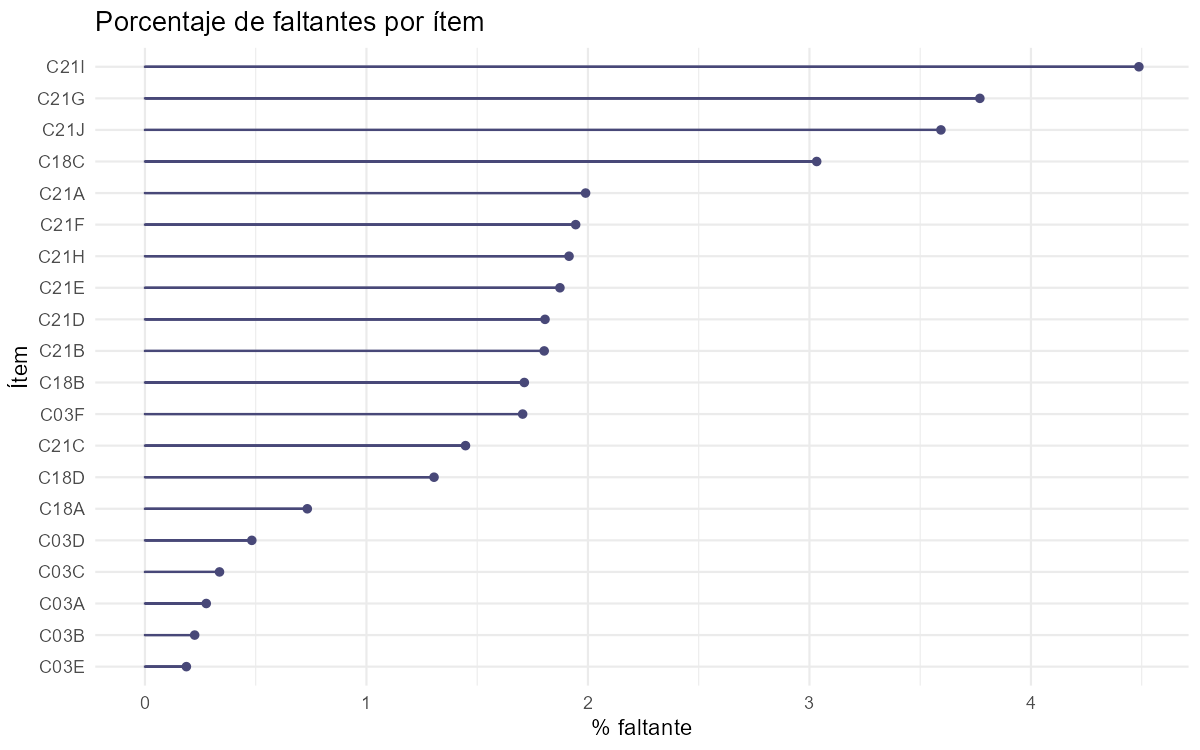
\includegraphics[width=0.65\textwidth]{act3_faltantes_por_item.png} 
    \caption{Porcentaje de datos faltantes por ítem en la base analítica ($n = 26.742$).}
    \label{fig:faltantes_item}
\end{figure}

Para formalizar la naturaleza del mecanismo de faltantes, se ejecutó la Prueba de Little (MCAR). El resultado arrojó un estadístico de prueba $\chi^2 = 17.677,7$ con $11.007$ grados de libertad y un valor $p < 0.001$, rechazando de forma contundente la hipótesis de que los datos son Faltantes Completamente al Azar (MCAR). Se asume por tanto un mecanismo de Faltantes al Azar (MAR) o No al Azar (MNAR), descartando la eliminación por listwise sin corrección y recomendando métodos de información completa como Pairwise o FIML en la estimación del modelo estructural (Enders, 2022). La interacción visual de patrones se ilustra en la Figura \ref{fig:patron_upset}.

\begin{figure}[H]
    \centering
    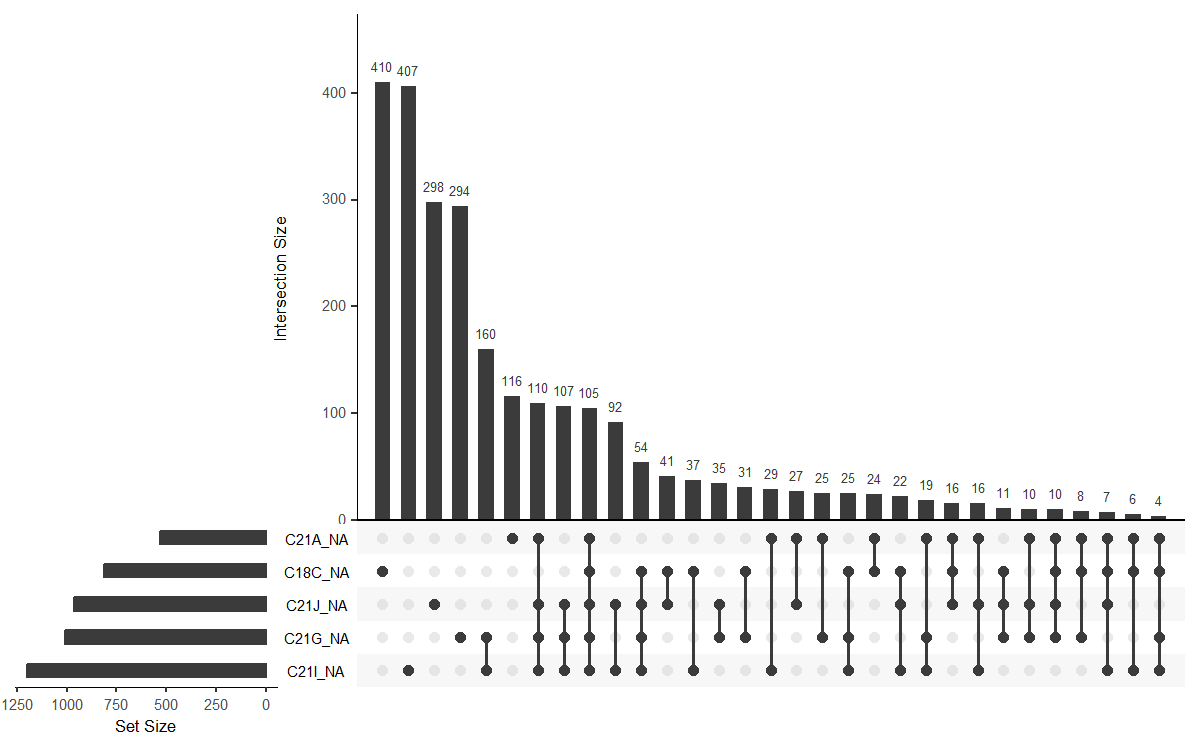
\includegraphics[width=0.65\textwidth]{act3_patron_faltantes.png} 
    \caption{Gráfico de intersección (UpSet) para los patrones de faltantes dominantes.}
    \label{fig:patron_upset}
\end{figure}

\subsection{Atípicos Univariados, Multivariados y Straightlining}

\begin{itemize}[leftmargin=*, itemsep=2pt]
    \item \textbf{Atípicos Univariados ($z$-robusto):} Al calcular el puntaje $z$ robusto basado en la Mediana y la Desviación Absoluta respecto a la Mediana ($\text{MAD} = \text{median}(|x_i - \text{median}(x)|)$), la presencia de MAD = 0 en ítems ordinales con alta concentración de respuestas impidió detectar atípicos por esta vía. Los diagramas de caja (Figura \ref{fig:boxplots}) reflejan distribuciones muy sesgadas hacia las puntuaciones altas.
    \item \textbf{Atípicos Multivariados (Mahalanobis):} Sobre los $23.497$ casos completos, se calculó la distancia de Mahalanobis $D^2$. Fijando un umbral estricto con $\chi^2_{0.999, df=20} = 45.31$, se identificaron $2.261$ observaciones atípicas multivariadas ($9.62\%$). Como se observa en la Figura \ref{fig:mahalanobis}, estas respuestas no representan errores de digitalización sino patrones extremos legítimos de alta o baja evaluación institucional.
    \item \textbf{Patrones de Invarianza (Straightlining):} Se detectaron $1.011$ observaciones ($3.78\%$) que respondieron de manera idéntica el valor en todos los ítems (el $62.3\%$ fijó la categoría 5 y el $32.5\%$ la categoría 4). Se decidió conservar la totalidad de estas observaciones para preservar la representatividad muestral y realizar análisis de sensibilidad en la Fase 2.
\end{itemize}

\begin{figure}[H]
    \centering
    \begin{subfigure}[b]{0.48\textwidth}
        \centering
        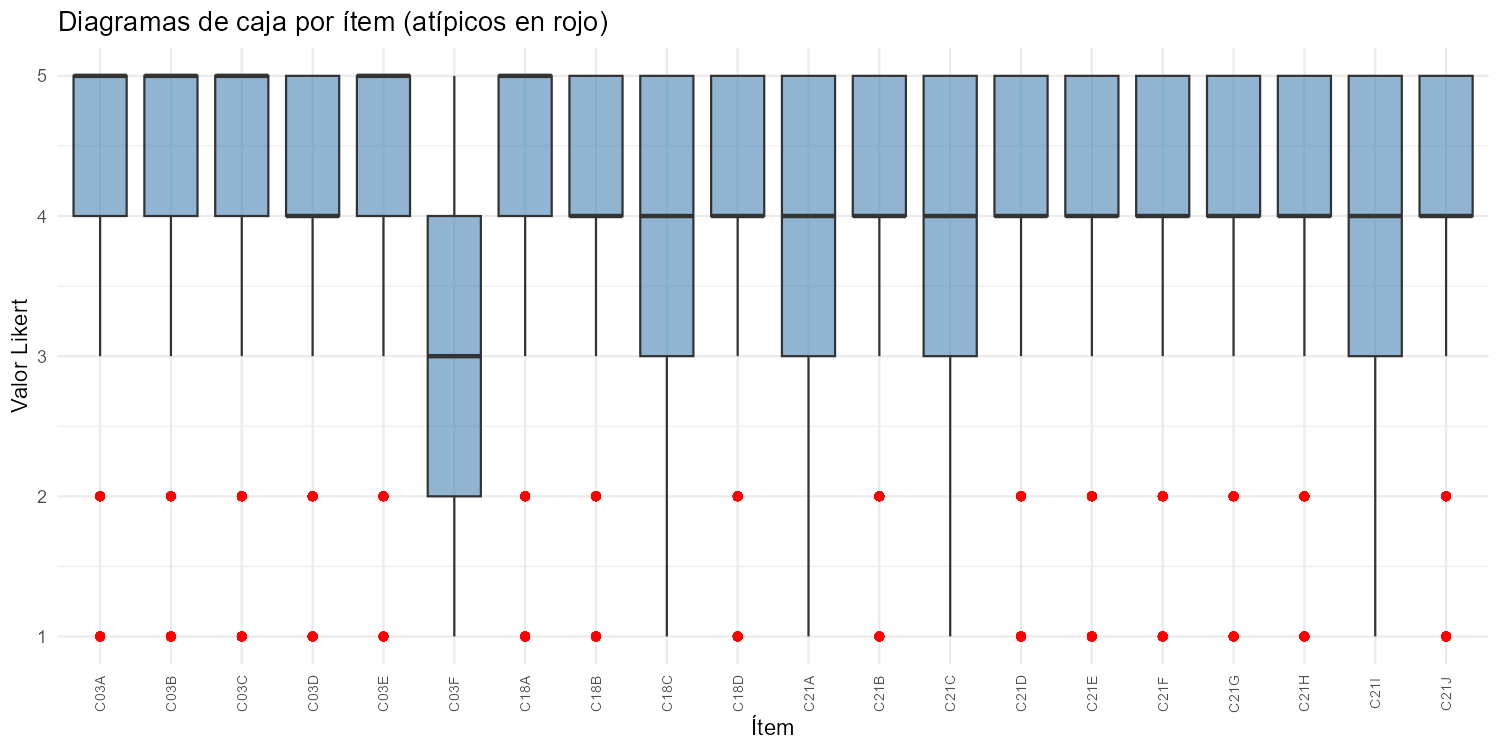
\includegraphics[width=\textwidth]{act3_boxplots.png}
        \caption{Diagramas de caja por ítem.}
        \label{fig:boxplots}
    \end{subfigure}
    \hfill
    \begin{subfigure}[b]{0.48\textwidth}
        \centering
        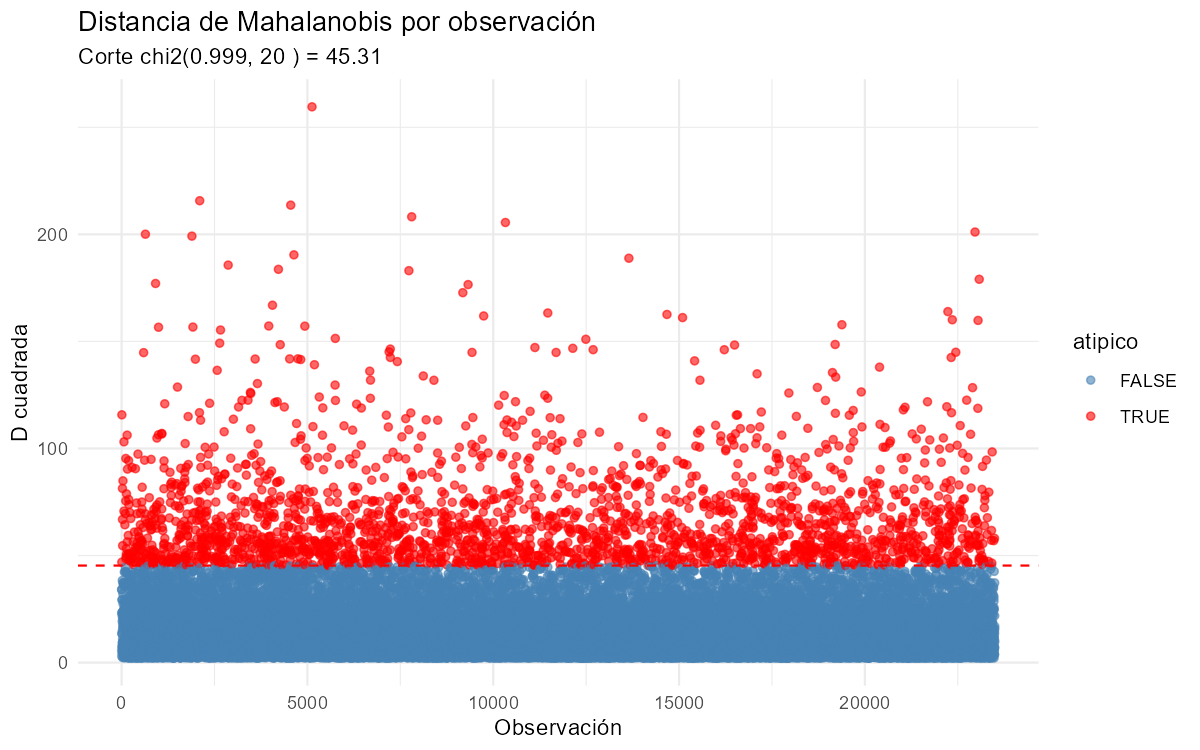
\includegraphics[width=\textwidth]{act3_mahalanobis.png}
        \caption{Distancia de Mahalanobis ($D^2$).}
        \label{fig:mahalanobis}
    \end{subfigure}
    \caption{Diagnóstico univariado y multivariado de valores extremos en la muestra.}
\end{figure}

% ==========================================
% 6. DESCRIPCIÓN Y DISTRIBUCIÓN DE INDICADORES
% ==========================================
\section{Descripción y Distribución de los Indicadores}

\subsection{Análisis Descriptivo Univariado}

Los 19 indicadores exhiben promedios sensiblemente altos (Tabla \ref{tab:descriptivos_19items}), fluctuando entre $3.89$ (C21A: asignación equitativa de cargas) y $4.62$ (C03E: esfuerzo por cumplir el trabajo). Las desviaciones estándar oscilan entre $0.58$ y $1.10$.

\begin{table}[H]
\centering
\footnotesize 
\caption{Estadísticos descriptivos completos para los 19 indicadores analíticos ($n = 26.742$).}
\label{tab:descriptivos_19items}
\begin{tabularx}{\textwidth}{l l c c c c c c}
\toprule
\textbf{Constructo} & \textbf{Item} & \textbf{Media} & \textbf{D.E.} & \textbf{Mediana} & \textbf{Asimetría} & \textbf{Curtosis} & \textbf{\% Techo (5)} \\
\midrule
\multirow{4}{*}{\shortstack[l]{Clima\\Laboral}} 
& C18A & 4.37 & 0.79 & 5.00 & -1.54 & 2.97 & 51.6\% \\
& C18B & 4.18 & 0.87 & 4.00 & -1.17 & 1.45 & 41.0\% \\
& C18C & 3.92 & 0.96 & 4.00 & -0.85 & 0.55 & 30.0\% \\
& C18D & 4.11 & 0.86 & 4.00 & -1.09 & 1.57 & 35.1\% \\
\midrule
\multirow{10}{*}{Liderazgo} 
& C21A & 3.89 & 1.10 & 4.00 & -0.98 & 0.29 & 33.5\% \\
& C21B & 4.02 & 1.02 & 4.00 & -1.15 & 0.98 & 36.9\% \\
& C21C & 3.95 & 1.07 & 4.00 & -1.01 & 0.52 & 35.7\% \\
& C21D & 4.03 & 0.99 & 4.00 & -1.13 & 1.06 & 37.0\% \\
& C21E & 4.03 & 1.04 & 4.00 & -1.18 & 1.02 & 38.7\% \\
& C21F & 4.00 & 1.07 & 4.00 & -1.11 & 0.73 & 38.5\% \\
& C21G & 4.05 & 0.98 & 4.00 & -1.13 & 1.14 & 37.7\% \\
& C21H & 3.99 & 1.04 & 4.00 & -1.09 & 0.81 & 36.7\% \\
& C21I & 3.90 & 1.04 & 4.00 & -0.89 & 0.41 & 32.2\% \\
& C21J & 4.22 & 0.95 & 4.00 & -1.48 & 2.22 & 46.5\% \\
\midrule
\multirow{5}{*}{\shortstack[l]{Satisfacción\\Laboral}} 
& C03A & 4.41 & 0.77 & 5.00 & -1.61 & 3.41 & 53.9\% \\
& C03B & 4.58 & 0.68 & 5.00 & -1.99 & 5.27 & 66.2\% \\
& C03C & 4.48 & 0.80 & 5.00 & -1.85 & 3.84 & 62.3\% \\
& C03D & 4.05 & 1.03 & 4.00 & -1.18 & 0.95 & 39.6\% \\
& C03E & 4.62 & 0.58 & 5.00 & -1.70 & 4.66 & 65.8\% \\
\bottomrule
\end{tabularx}
\end{table}

\subsection{Efectos Piso y Techo}

Se evaluó la presencia de concentraciones anómalas en los extremos de la escala Likert (piso = valor 1, techo = valor 5), adoptando el umbral crítico del 15\% establecido en la literatura. La Figura \ref{fig:piso_techo} evidencia severos efectos techo en la totalidad de los indicadores: en el constructo de Satisfacción, el porcentaje de respuestas en la máxima categoría alcanza un $66.2\%$ en C03B y un $65.8\%$ en C03E. En contraste, el efecto piso es marginal ($< 4.41\%$). Esta asimetría refleja deseabilidad social en encuestas del sector público.

\begin{figure}[H]
    \centering
    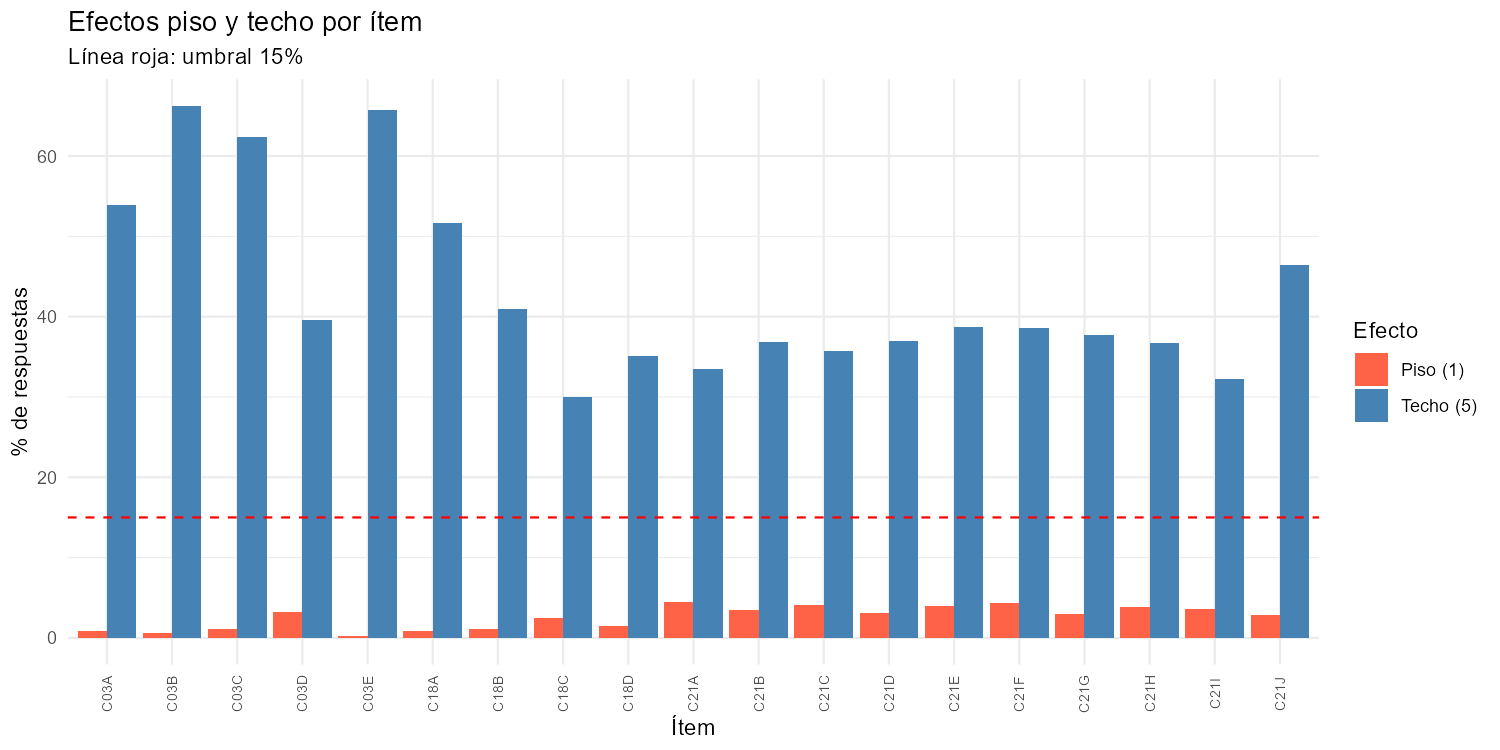
\includegraphics[width=0.65\textwidth]{act4_piso_techo.png} 
    \caption{Porcentaje de efectos piso (categoría 1) y techo (categoría 5) por ítem.}
    \label{fig:piso_techo}
\end{figure}

\begin{figure}[H]
    \centering
    \begin{subfigure}[b]{0.48\textwidth}
        \centering
        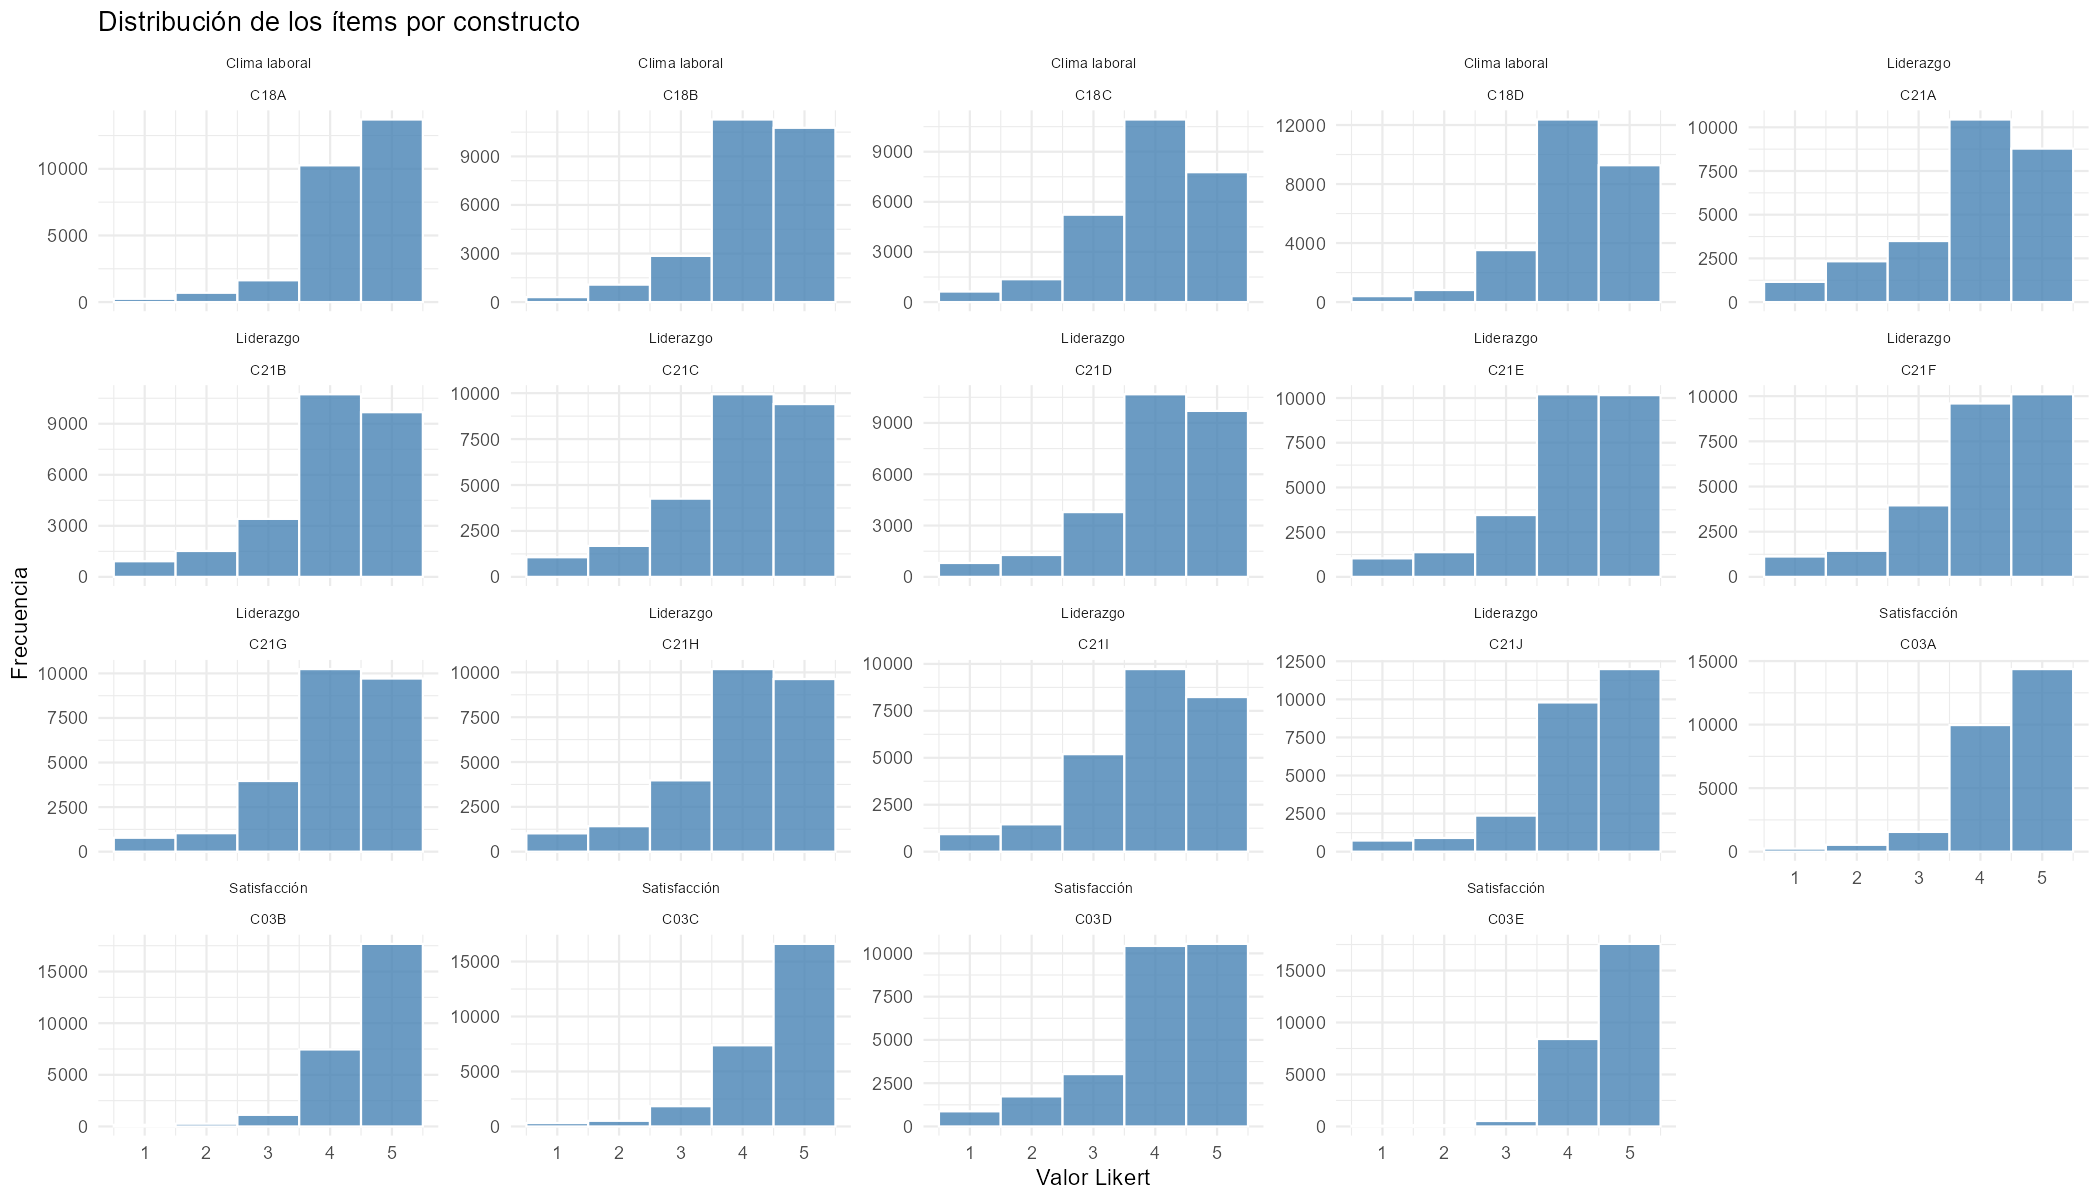
\includegraphics[width=\textwidth]{act4_histogramas.png}
        \caption{Histogramas de frecuencia Likert.}
        \label{fig:histogramas}
    \end{subfigure}
    \hfill
    \begin{subfigure}[b]{0.48\textwidth}
        \centering
        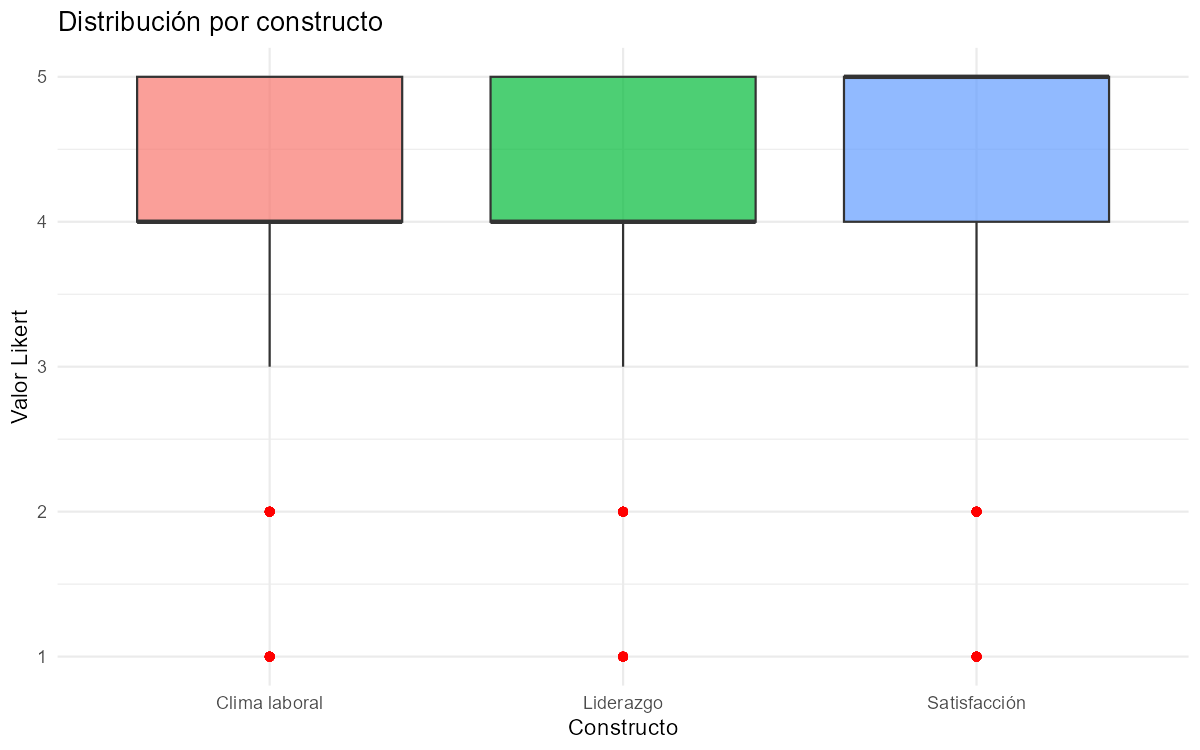
\includegraphics[width=\textwidth]{act4_boxplot_constructo.png}
        \caption{Distribución por constructo latente.}
        \label{fig:box_constructo}
    \end{subfigure}
    \caption{Comportamiento gráfico de las distribuciones univariadas y por dimensión.}
\end{figure}

\subsection{Evaluación de Normalidad Multivariada y Selección del Estimador}

Aunque los coeficientes univariados de asimetría ($|Skew| \le 1.99$) y curtosis ($|Kurt| \le 5.27$) se encuentran formalmente dentro de los límites permisibles para distribuciones continuas ($|Skew| < 2, |Kurt| < 7$; West et al., 1995), la naturaleza ordinal Likert de 5 puntos exige la comprobación de la Normalidad Multivariada.

Se ejecutó la Prueba de Asimetría y Curtosis Multivariada de Mardia sobre las $23.760$ observaciones sin ningún dato faltante. Los resultados confirmaron una severa desviación del supuesto gaussiano multivariado:

\begin{itemize}[itemsep=2pt]
    \item \textbf{Asimetría Multivariada de Mardia:} $b_{1,p} = 47.2086$, con un estadístico de prueba $\chi^2 = 186.946,1$ ($df = 1.330, p < 0.001$).
    \item \textbf{Curtosis Multivariada de Mardia:} $b_{2,p} = 762.5252$, con un estadístico estandarizado $z = 991.8051$ ($p < 0.001$). El valor esperado de $b_{2,p}$ bajo normalidad perfecta es $p(p+2) = 19(21) = 399$.
\end{itemize}

\begin{table}[H]
\centering
\caption{Criterio de decisión para la selección del estimador en la Fase 2.}
\label{tab:decision_estimador}
\footnotesize
\begin{tabularx}{\textwidth}{l X}
\toprule
\textbf{Criterio Evaluado} & \textbf{Diagnóstico Empírico / Justificación} \\
\midrule
Tipo de indicadores & Ordinales discretos (Escala Likert de 5 niveles). \\
Evaluación de Normalidad & Se rechaza categóricamente la Normalidad Multivariada (Mardia $p < 0.001$). \\
Inadecuación de ML & El estimador Máxima Verosimilitud (ML) atenúa las cargas factoriales y distorsiona los errores estándar bajo datos ordinales sesgados (Li, 2016). \\
\textbf{Estimador Seleccionado} & \textbf{WLSMV} (\textit{Weighted Least Squares Means and Variance Adjusted}). \\
Propiedades de WLSMV & Trabaja directamente sobre la matriz de correlaciones policóricas y umbrales (\textit{thresholds}), proporcionando estimaciones e índices de ajuste corregidos por no normalidad (Li, 2016). \\
\bottomrule
\end{tabularx}
\end{table}

% ==========================================
% 7. ASOCIACIÓN Y ESTRUCTURA EXPLORATORIA
% ==========================================
\section{Análisis de Asociación y Estructura Exploratoria}

\subsection{Matriz de Correlaciones Policóricas y Validez de Discriminante}

Dado el carácter ordinal de los ítems, se calculó la matriz de correlaciones policóricas ($19 \times 19$). La matriz resultó ser estrictamente positiva definida, con un determinante de $\det(\mathbf{R}_{pol}) = 2.305 \times 10^{-9}$.

La Figura \ref{fig:mapa_calor} ilustra la matriz policórica ordenada por constructos. Se observa una marcada ordenación en bloques diagonales, con correlaciones dentro de los constructos sustancialmente superiores a las correlaciones entre constructos diferentes, aportando evidencia preliminar de validez convergente y discriminante.

\begin{figure}[H]
    \centering
    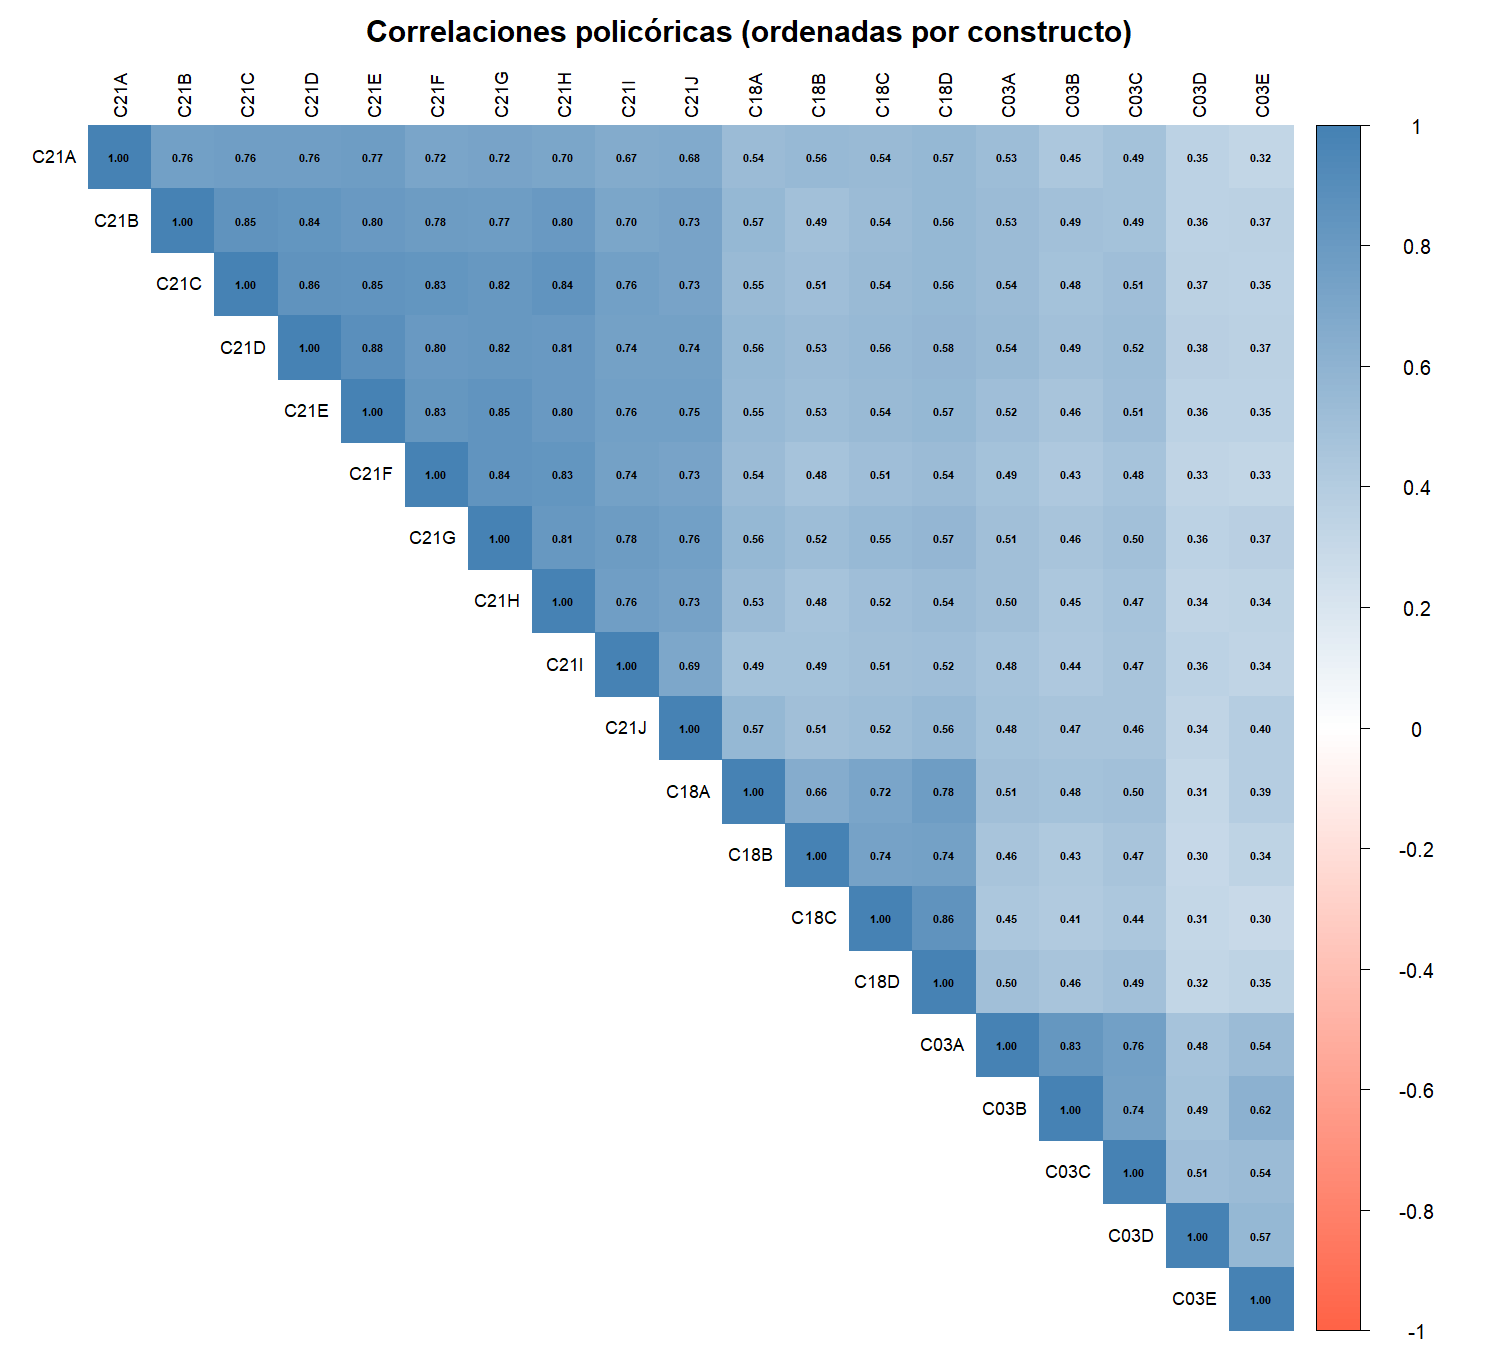
\includegraphics[width=0.65\textwidth]{act5_mapa_calor_poli.png} 
    \caption{Mapa de calor de correlaciones policóricas ordenadas por constructo.}
    \label{fig:mapa_calor}
\end{figure}

\begin{table}[H]
\centering
\footnotesize
\caption{Promedio de correlaciones policóricas dentro y entre constructos.}
\label{tab:correlaciones_resumen}
\begin{tabular}{lc | lc}
\toprule
\textbf{Correlación Intra-Constructo} & \textbf{Promedio $r_{pol}$} & \textbf{Correlación Inter-Constructo} & \textbf{Promedio $r_{pol}$} \\
\midrule
Liderazgo -- Liderazgo & 0.777 & Liderazgo -- Clima Laboral & 0.536 \\
Clima Laboral -- Clima Laboral & 0.748 & Liderazgo -- Satisfacción & 0.435 \\
Satisfacción -- Satisfacción & 0.606 & Clima Laboral -- Satisfacción & 0.412 \\
\bottomrule
\end{tabular}
\end{table}

\subsection{Análisis de Confiabilidad y Consistencia Interna}

Se calcularon los coeficientes $\alpha$ de Cronbach (1951) y $\omega$ de McDonald (1999) para cada dimensión, complementados con la correlación ítem-resto ($r_{i-r}$). La totalidad de las dimensiones superó con holgura los umbrales psicométricos estándar ($\ge 0.70$).

\begin{table}[H]
\centering
\footnotesize
\caption{Resumen de consistencia interna y rangos ítem-resto por constructo.}
\label{tab:confiabilidad}
\begin{tabular}{l c c c c}
\toprule
\textbf{Constructo Latente} & \textbf{Nº Ítems} & \textbf{$\alpha$ de Cronbach} & \textbf{$\omega$ de McDonald} & \textbf{Rango Ítem-Resto ($r_{i-r}$)} \\
\midrule
Liderazgo ($\xi_1$) & 10 & 0.956 & 0.958 & 0.705 -- 0.867 \\
Clima Laboral ($\eta_1$) & 4 & 0.876 & 0.881 & 0.674 -- 0.815 \\
Satisfacción Laboral ($\eta_2$) & 5 & 0.795 & 0.822 & 0.463 -- 0.686 \\
\bottomrule
\end{tabular}
\end{table}

\subsection{Análisis Factorial Exploratorio (AFE)}

La adecuación muestral para la factorización fue confirmada mediante el test KMO ($\text{MSA Global} = 0.963$, calificación "excelente") y la Prueba de Esfericidad de Bartlett ($\chi^2 = 531.682,7, df = 171, p < 0.001$). El Análisis Paralelo de Horn (Figura \ref{fig:analisis_paralelo}) sugirió retener 3 factores principales.

\begin{figure}[H]
    \centering
    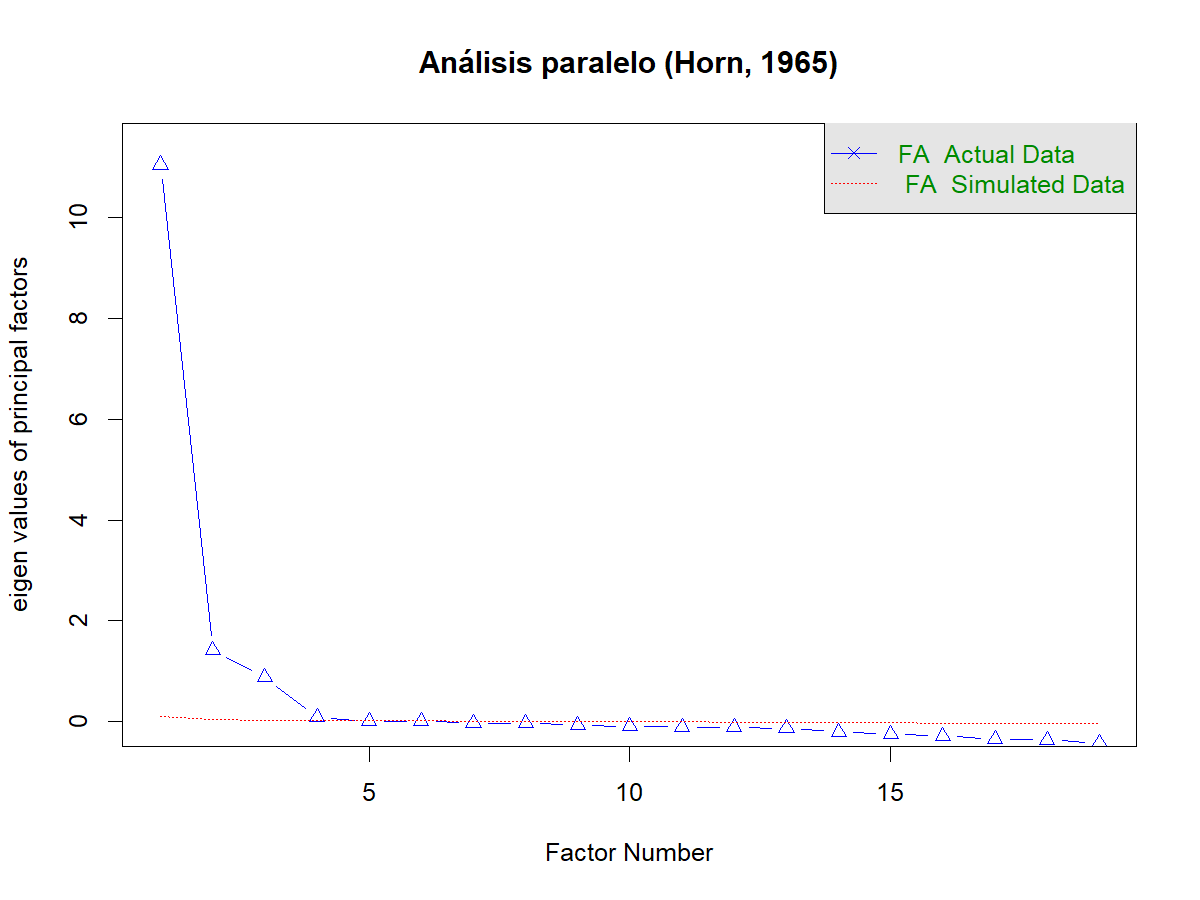
\includegraphics[width=0.65\textwidth]{act5_analisis_paralelo.png} 
    \caption{Análisis paralelo de Horn (1965) para la determinación del número de factores.}
    \label{fig:analisis_paralelo}
\end{figure}

Se estimó el AFE con 3 factores utilizando extracción por Mínimos Residuos (\texttt{minres}) y rotación oblicua (\texttt{oblimin}). Los resultados (Figura \ref{fig:cargas_afe}) revelan una estructura factorial pura: \textbf{los 19 ítems cargaron de forma dominadora e inequívoca en sus respectivos constructos hipotetizados} (MR3 = Liderazgo, MR1 = Clima, MR2 = Satisfacción), sin cargas cruzadas significativamente elevadas ($> 0.30$). El modelo de 3 factores explica el \textbf{$73.5\%$ de la varianza total acumulada}.

\begin{figure}[H]
    \centering
    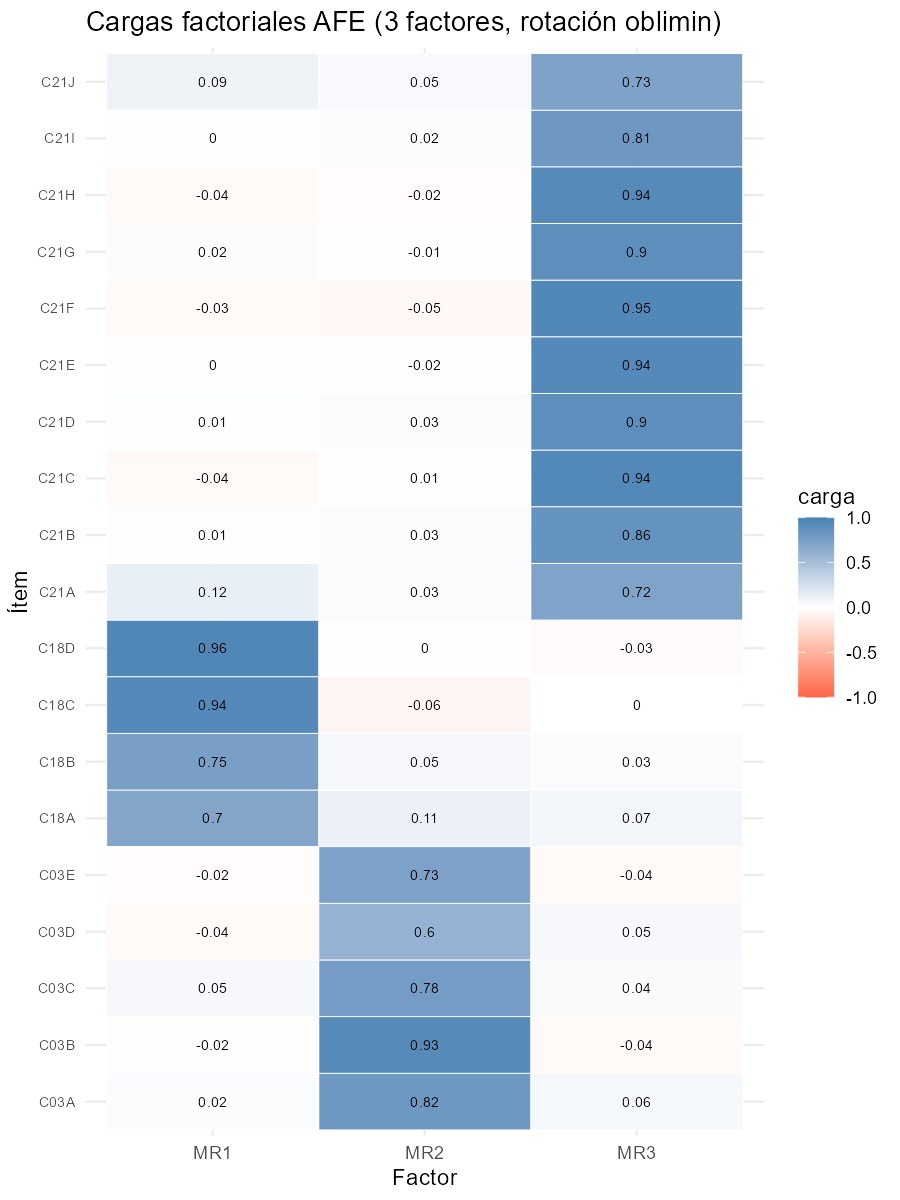
\includegraphics[width=0.55\textwidth]{act5_cargas_afe.png} 
    \caption{Matriz de cargas factoriales del AFE de 3 factores con rotación oblimin.}
    \label{fig:cargas_afe}
\end{figure}

% ==========================================
% 8. ESPECIFICACIÓN DEL MODELO Y NOTACIÓN LISREL
% ==========================================
\section{Especificación del Modelo Estructural y Notación Matricial}

\subsection{Formulación en Notación LISREL}

El modelo de mediación parcial propuesto ($M_1$) se especifica mediante el sistema formal de ecuaciones estructurales LISREL:

\begin{equation}
\mathbf{x} = \mathbf{\Lambda}_x \xi_1 + \boldsymbol{\delta}
\end{equation}

\begin{equation}
\mathbf{y} = \mathbf{\Lambda}_y \boldsymbol{\eta} + \boldsymbol{\epsilon}
\end{equation}

\begin{equation}
\boldsymbol{\eta} = \mathbf{B} \boldsymbol{\eta} + \mathbf{\Gamma} \xi_1 + \boldsymbol{\zeta}
\end{equation}

Desglosando en términos matriciales explícitos para los 19 indicadores:

\begin{equation}
\begin{bmatrix} C21A \\ C21B \\ C21C \\ C21D \\ C21E \\ C21F \\ C21G \\ C21H \\ C21I \\ C21J \end{bmatrix} = \begin{bmatrix} 1 \\ \lambda^x_{2,1} \\ \lambda^x_{3,1} \\ \lambda^x_{4,1} \\ \lambda^x_{5,1} \\ \lambda^x_{6,1} \\ \lambda^x_{7,1} \\ \lambda^x_{8,1} \\ \lambda^x_{9,1} \\ \lambda^x_{10,1} \end{bmatrix} [\text{Liderazgo}] + \begin{bmatrix} \delta_1 \\ \delta_2 \\ \delta_3 \\ \delta_4 \\ \delta_5 \\ \delta_6 \\ \delta_7 \\ \delta_8 \\ \delta_9 \\ \delta_{10} \end{bmatrix}
\end{equation}

\begin{equation}
\begin{bmatrix} C18A \\ C18B \\ C18C \\ C18D \\ C03A \\ C03B \\ C03C \\ C03D \\ C03E \end{bmatrix} = \begin{bmatrix} 1 & 0 \\ \lambda^y_{2,1} & 0 \\ \lambda^y_{3,1} & 0 \\ \lambda^y_{4,1} & 0 \\ 0 & 1 \\ 0 & \lambda^y_{6,2} \\ 0 & \lambda^y_{7,2} \\ 0 & \lambda^y_{8,2} \\ 0 & \lambda^y_{9,2} \end{bmatrix} \begin{bmatrix} \text{Clima} \\ \text{Satisfacción} \end{bmatrix} + \begin{bmatrix} \epsilon_1 \\ \epsilon_2 \\ \epsilon_3 \\ \epsilon_4 \\ \epsilon_5 \\ \epsilon_6 \\ \epsilon_7 \\ \epsilon_8 \\ \epsilon_9 \end{bmatrix}
\end{equation}

\begin{equation}
\begin{bmatrix} \text{Clima} \\ \text{Satisfacción} \end{bmatrix} = \begin{bmatrix} 0 & 0 \\ \beta_{21} & 0 \end{bmatrix} \begin{bmatrix} \text{Clima} \\ \text{Satisfacción} \end{bmatrix} + \begin{bmatrix} \gamma_{11} \\ \gamma_{21} \end{bmatrix} [\text{Liderazgo}] + \begin{bmatrix} \zeta_1 \\ \zeta_2 \end{bmatrix}
\end{equation}

\begin{table}[H]
\centering
\caption{Especificación de matrices del modelo LISREL, dimensiones y recuento de parámetros.}
\label{tab:matrices_lisrel}
\footnotesize
\begin{tabularx}{\textwidth}{l c c c X}
\toprule
\textbf{Matriz LISREL} & \textbf{Dimensión} & \textbf{Elem. Libres} & \textbf{Elem. Fijos} & \textbf{Descripción y Fijación de Escala} \\
\midrule
$\mathbf{\Lambda}_x$ & $10 \times 1$ & 9 & 1 & Cargas de Liderazgo (C21A fija en 1 como marcador de escala). \\
$\mathbf{\Lambda}_y$ & $9 \times 2$ & 7 & 11 & Cargas de Clima (C18A=1) y Satisfacción (C03A=1); sin cargas cruzadas. \\
$\mathbf{B}$ & $2 \times 2$ & 1 & 3 & Efecto $\beta_{21}$ (Clima $\rightarrow$ Satisfacción) libre; resto ceros. \\
$\mathbf{\Gamma}$ & $2 \times 1$ & 2 & 0 & Efectos directos $\gamma_{11}$ (Liderazgo $\rightarrow$ Clima) y $\gamma_{21}$ libres. \\
$\mathbf{\Phi}$ & $1 \times 1$ & 1 & 0 & Varianza de la latente exógena Liderazgo libre. \\
$\mathbf{\Psi}$ & $2 \times 2$ & 2 & 2 & Varianzas de perturbación $\zeta_1, \zeta_2$ libres; covarianza fija en 0. \\
$\mathbf{\Theta}_\epsilon$ & $9 \times 9$ & 9 & 72 & Varianzas de error para $y$ libres; covarianzas fijas en 0. \\
$\mathbf{\Theta}_\delta$ & $10 \times 10$ & 10 & 90 & Varianzas de error para $x$ libres; covarianzas fijas en 0. \\
\bottomrule
\end{tabularx}
\end{table}

\subsection{Evaluación Formal de Identificabilidad}

Para verificar que el modelo se encuentra adecuadamente identificado, calculamos la regla del $t$:

\begin{itemize}[leftmargin=*, itemsep=2pt]
    \item \textbf{Número de indicadores ($k$):} $k = 19$ ítems analíticos.
    \item \textbf{Momentos muestrales disponibles ($p^*$):} $p^* = \frac{k(k+1)}{2} = \frac{19(20)}{2} = 190$ covarianzas/varianzas distintas.
    \item \textbf{Parámetros libres a estimar ($t$):} $t = 9 (\mathbf{\Lambda}_x) + 7 (\mathbf{\Lambda}_y) + 1 (\mathbf{B}) + 2 (\mathbf{\Gamma}) + 1 (\mathbf{\Phi}) + 2 (\mathbf{\Psi}) + 9 (\mathbf{\Theta}_\epsilon) + 10 (\mathbf{\Theta}_\delta) = 41$ parámetros libres.
    \item \textbf{Grados de Libertad ($gl$):} $gl = p^* - t = 190 - 41 = 149$ grados de libertad.
\end{itemize}

Dado que $gl = 149 \ge 0$, el modelo está \textbf{sobreidentificado}. Adicionalmente, se satisface la \textbf{Regla de los Tres Indicadores} ($\ge 3$ ítems por latente) y la \textbf{Regla de Recursividad} ($\mathbf{B}$ es triangular inferior con ceros en la diagonal y sin bucles de retroalimentación).

\subsection{Diagramas de Caminos y Modelo Rival}

En las Figuras \ref{fig:diagrama_propuesto} y \ref{fig:diagrama_rival} se presentan las representaciones gráficas del modelo propuesto $M_1$ y del modelo rival de comparación $M_2$ (sin efecto mediador de Clima a Satisfacción).

\begin{figure}[H]
    \centering
    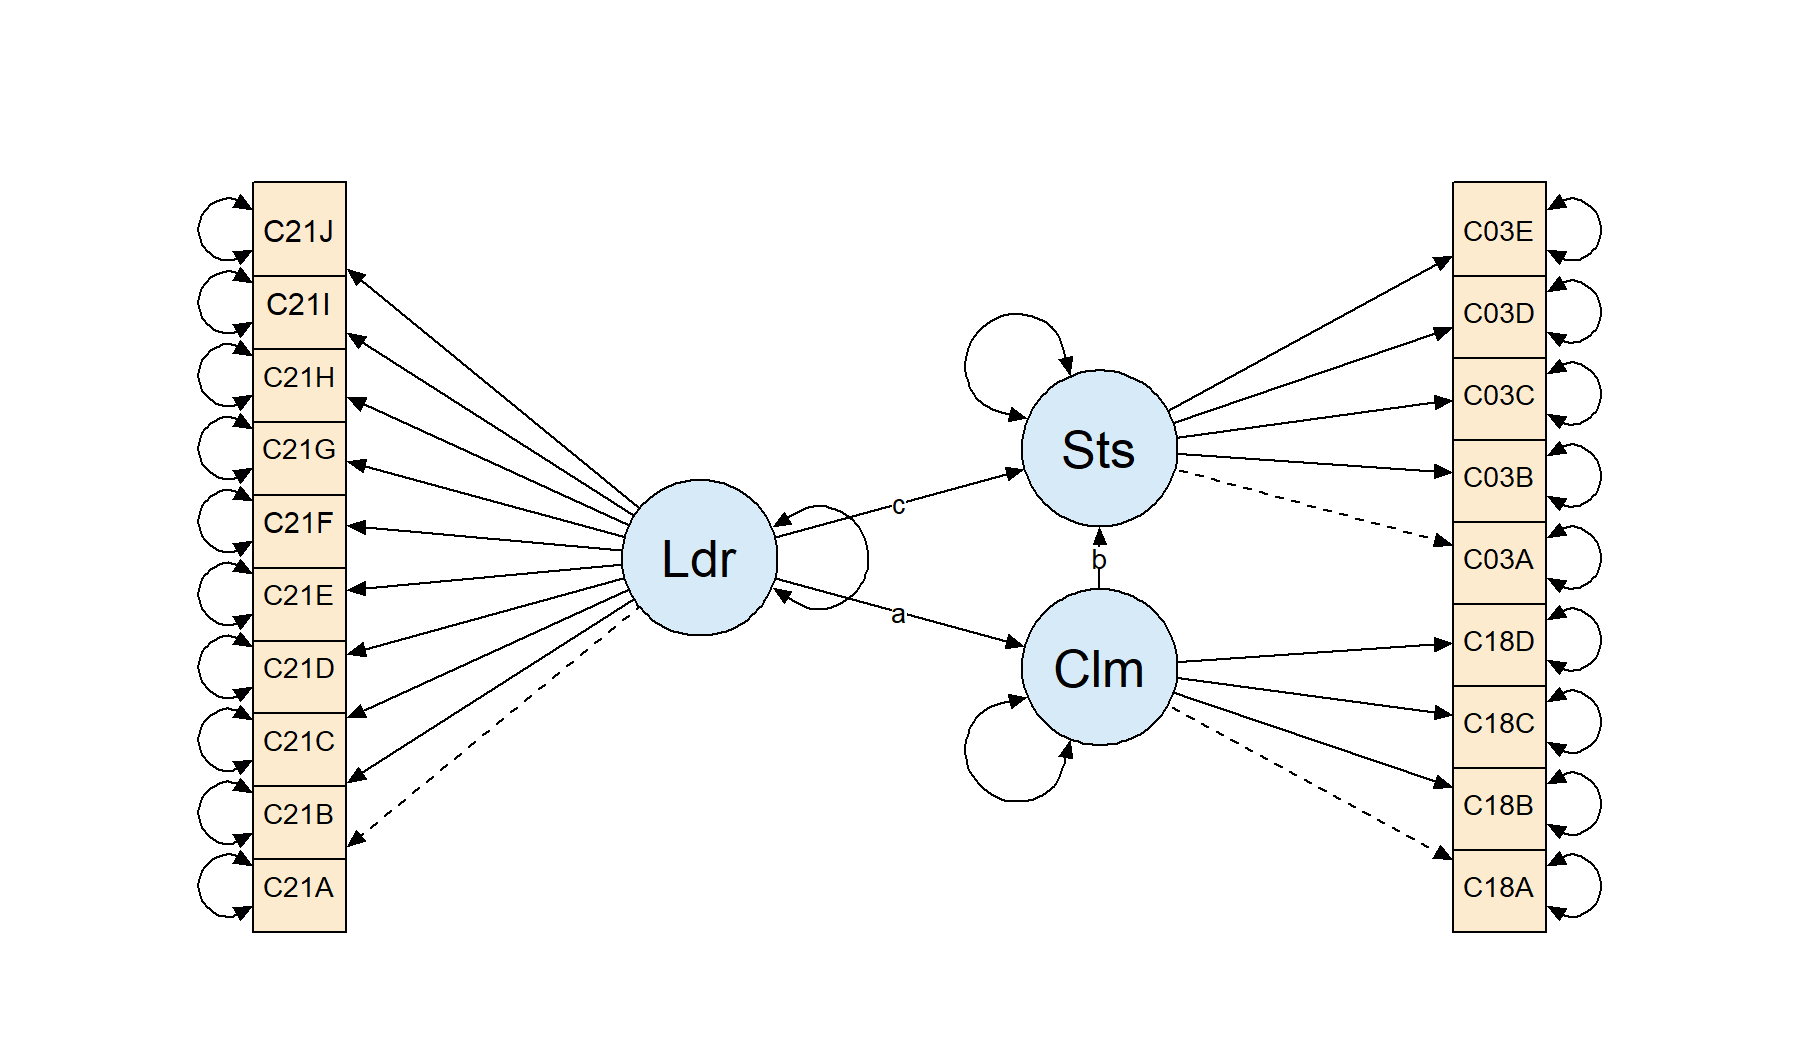
\includegraphics[width=0.75\textwidth]{act6_diagrama_caminos.png} 
    \caption{Diagrama de caminos del modelo de mediación propuesto ($M_1$) especificado en \texttt{semPlot}.}
    \label{fig:diagrama_propuesto}
\end{figure}

\begin{figure}[H]
    \centering
    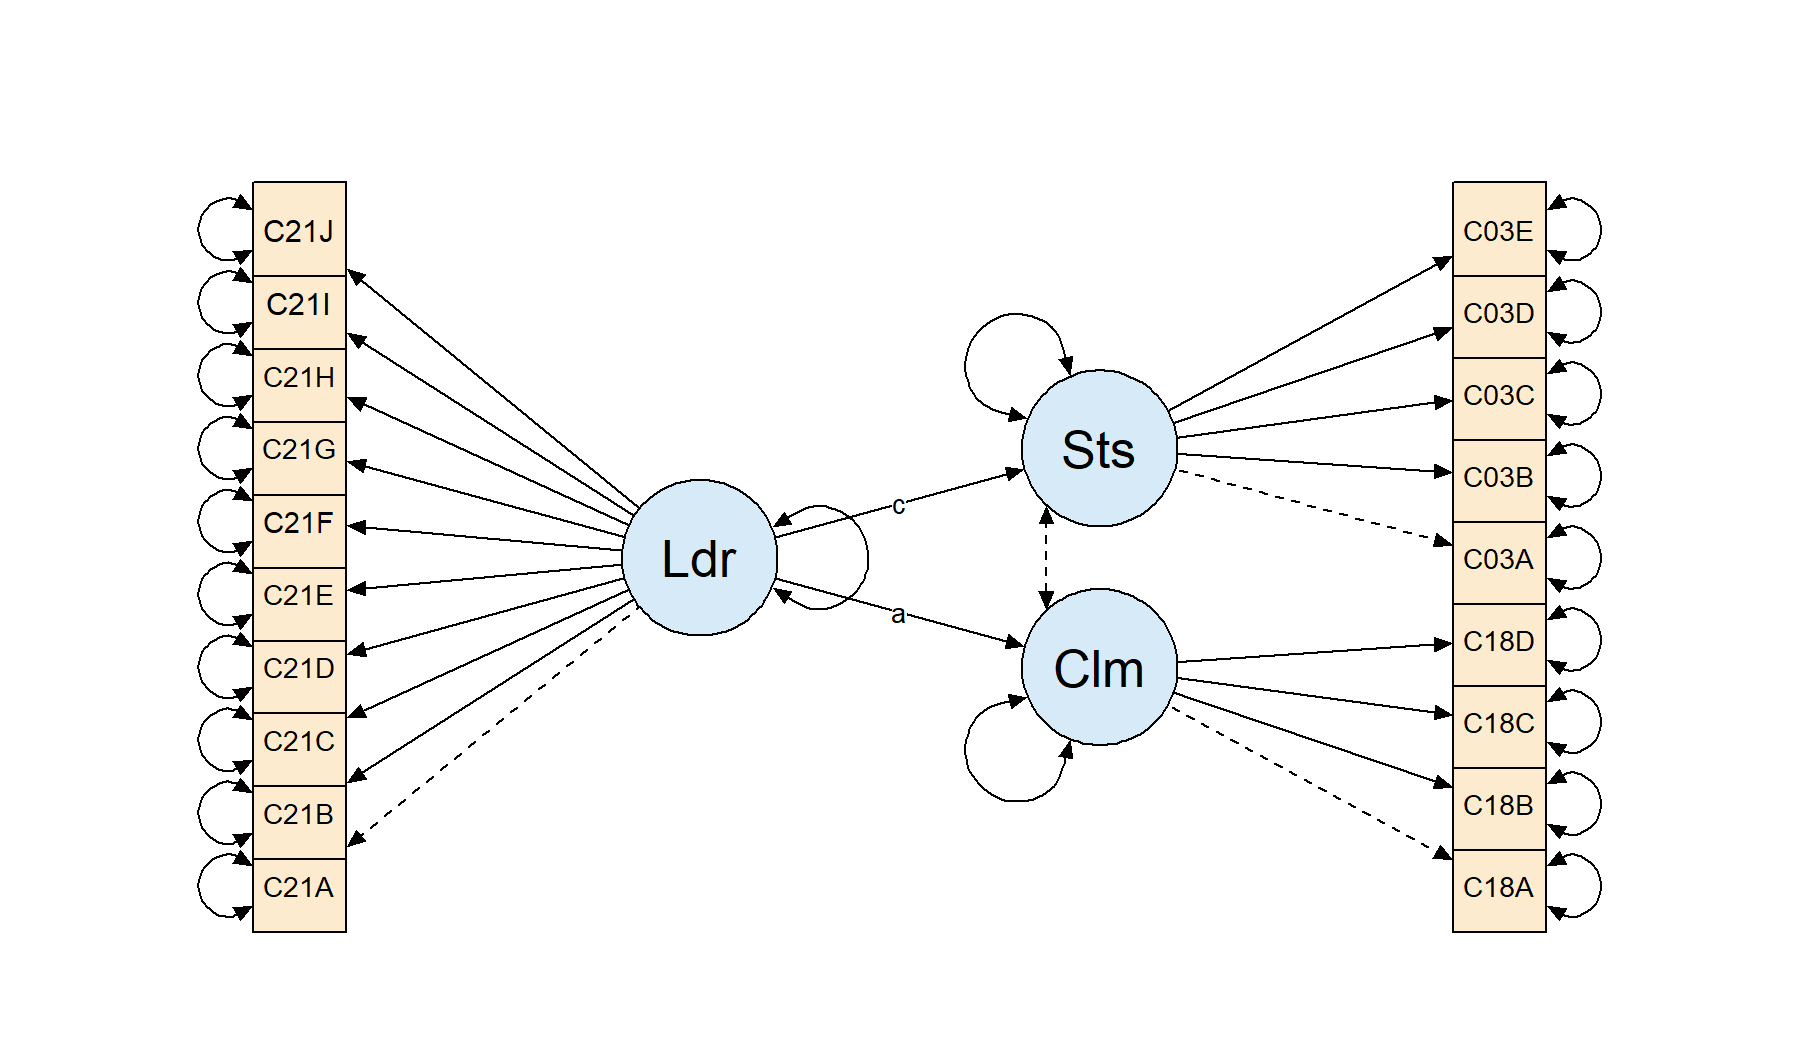
\includegraphics[width=0.75\textwidth]{act6_diagrama_rival.png} 
    \caption{Diagrama de caminos del modelo rival de comparación directos sin mediación ($M_2$).}
    \label{fig:diagrama_rival}
\end{figure}

\subsection{Sintaxis Formal en lavaan}

La sintaxis del modelo propuesto $M_1$ codificada para su posterior ejecución en R se detalla a continuación:

\begin{lstlisting}[caption={Sintaxis del modelo de mediación propuesto ($M_1$) en \texttt{lavaan}.}, label={lst:modelo}]
# =====================================================================
# SINTAXIS LAVAAN: MODELO PROPUESTO DE MEDIACIÓN (M1)
# =====================================================================
modelo_propuesto <- '
  # --- Modelo de Medición ---
  Liderazgo    =~ C21A + C21B + C21C + C21D + C21E +
                  C21F + C21G + C21H + C21I + C21J
  Clima        =~ C18A + C18B + C18C + C18D
  Satisfaccion =~ C03A + C03B + C03C + C03D + C03E

  # --- Modelo Estructural ---
  Clima        ~ a*Liderazgo
  Satisfaccion ~ b*Clima + c*Liderazgo

  # --- Definición de Efectos ---
  indirecto    := a * b
  directo      := c
  total        := c + (a * b)
'
\end{lstlisting}

% ==========================================
% 9. CONCLUSIONES Y HOJA DE RUTA FASE 2
% ==========================================
\section{Conclusiones de la Fase 1 y Hoja de Ruta para la Fase 2}

\subsection{Conclusiones Principales}

\begin{enumerate}[leftmargin=*, itemsep=2pt]
    \item \textbf{Solidez Psicometría e Integridad:} El procesamiento sobre la base EDI 2025 del DANE confirmó la excelente calidad de la información. La depuración técnica corrigió la ambigüedad de la variable \texttt{CUIN} creando la llave \texttt{ID\_SERV}.
    \item \textbf{Estructura Latente Pura:} El AFE con correlaciones policóricas respaldó plenamente la validez de constructo y la convergencia de los 19 ítems en las tres dimensiones teóricas, alcanzando un $73.5\%$ de varianza explicada.
    \item \textbf{Decisión del Estimador:} El rechazo categórico de la normalidad multivariada mediante la prueba de Mardia ($p < 0.001$) impone el uso obligado del estimador \textbf{WLSMV} para la estimación confirmativa en la Fase 2.
    \item \textbf{Sobreidentificación Formal:} El modelo $M_1$ se encuentra matemáticamente identificado con $149$ grados de libertad, listo para el contraste empírico de las hipótesis $H_1$ a $H_4$.
\end{enumerate}

\subsection{Hoja de Ruta Metodológica para la Fase 2}

\begin{itemize}[leftmargin=*, itemsep=2pt]
    \item \textbf{Estimación Confirmativa:} Estimar los parámetros del modelo $M_1$ en \texttt{lavaan} declarando las variables como ordenadas (\texttt{ordered = TRUE}) con estimador \texttt{WLSMV}.
    \item \textbf{Evaluación de Ajuste Global:} Verificar los índices de ajuste robustos con los umbrales estándar de la literatura (Hu \& Bentler, 1999): $\text{CFI} \ge 0.95$, $\text{TLI} \ge 0.95$, $\text{RMSEA} \le 0.06$ y $\text{SRMR} \le 0.08$.
    \item \textbf{Comparación con Modelo Rival:} Comparar los índices de ajuste de $M_1$ frente a $M_2$ empleando la prueba de diferencia de Chi-cuadrado ajustada para WLSMV (\texttt{lavTestLRT}).
    \item \textbf{Inferencia de Efectos:} Evaluar los errores estándar obtenidos mediante \textit{bootstrapping} no paramétrico para validar la significancia estadística del efecto indirecto de mediación ($\text{indirecto} = a \cdot b$).
\end{itemize}

% ==========================================
% 10. REFERENCIAS BIBLIOGRÁFICAS
% ==========================================
\begin{thebibliography}{99}
\small 
\setlength{\itemsep}{0pt} 

\bibitem{avolio2004} Avolio, B. J., \& Bass, B. M. (2004). \textit{Multifactor Leadership Questionnaire (MLQ): Manual and sampler set} (3rd ed.). Mind Garden.

\bibitem{bollen1989} Bollen, K. A. (1989). \textit{Structural equations with latent variables}. John Wiley \& Sons.

\bibitem{carr2003} Carr, J. Z., Schmidt, A. M., Ford, J. K., \& DeShon, R. P. (2003). Climate perceptions matter: A meta-analytic path analysis relating hygienic and motivators to employee outcomes. \textit{Journal of Applied Psychology}, 88(4), 605--619.

\bibitem{cronbach1951} Cronbach, L. J. (1951). Coefficient alpha and the internal structure of tests. \textit{Psychometrika}, 16(3), 297--334.

\bibitem{dane2025} Departamento Administrativo Nacional de Estadística [DANE]. (2025). \textit{Encuesta sobre Ambiente y Desempeño Institucional (EDI) - Sector Público 2025: Ficha técnica y microdatos anonimizados}. DANE.

\bibitem{enders2022} Enders, C. K. (2022). \textit{Applied missing data analysis} (2nd ed.). Guilford Press.

\bibitem{holgado2010} Holgado-Tello, F. P., Chacón-Moscoso, S., Barbero-García, I., \& Vila-Abad, E. (2010). Polychoric versus Pearson correlations in exploratory and confirmatory factor analysis of ordinal variables. \textit{Quality \& Quantity}, 44(1), 153--166.

\bibitem{horn1965} Horn, J. L. (1965). A rationale and test for the number of factors in factor analysis. \textit{Psychometrika}, 30(2), 179--185.

\bibitem{hu1999} Hu, L. T., \& Bentler, P. M. (1999). Cutoff criteria for fit indexes in covariance structure analysis: Conventional criteria versus new alternatives. \textit{Structural Equation Modeling: A Multidisciplinary Journal}, 6(1), 1--55.

\bibitem{judge2004} Judge, T. A., \& Piccolo, R. F. (2004). Transformational and transactional leadership: A meta-analytic test of their relative validity. \textit{Journal of Applied Psychology}, 89(5), 755--768.

\bibitem{kline2023} Kline, R. B. (2023). \textit{Principles and practice of structural equation modeling} (5th ed.). Guilford Press.

\bibitem{li2016} Li, C. H. (2016). The performance of ML, DWLS, and WLS estimation with ordinal variables. \textit{Structural Equation Modeling: A Multidisciplinary Journal}, 23(3), 331--349.

\bibitem{little1988} Little, R. J. A. (1988). A test of missing completely at random for multivariate data with missing values. \textit{Journal of the American Statistical Association}, 83(404), 1198--1202.

\bibitem{maccallum1993} MacCallum, R. C., Wegener, D. T., Uchino, B. N., \& Fabrigar, L. R. (1993). The problem of equivalent models in applications of covariance structure analysis. \textit{Psychological Bulletin}, 114(1), 185--199.

\bibitem{mardia1970} Mardia, K. V. (1970). Measures of multivariate skewness and kurtosis with applications. \textit{Biometrika}, 57(3), 519--530.

\bibitem{mcdonald1999} McDonald, R. P. (1999). \textit{Test theory: A unified treatment}. Lawrence Erlbaum Associates.

\bibitem{parker2003} Parker, C. P., Baltes, B. B., Young, S. A., Huff, J. W., Altmann, R. A., Lacost, H. A., \& Roberts, J. E. (2003). Relationships between psychological climate perceptions and work outcomes: A meta-analytic review. \textit{Journal of Organizational Behavior}, 24(4), 389--416.

\bibitem{schneider2013} Schneider, B., Ehrhart, M. G., \& Macey, W. H. (2013). Organizational climate and culture. \textit{Annual Review of Psychology}, 64, 361--388.

\bibitem{walumbwa2008} Walumbwa, F. O., Avolio, B. J., \& Zhu, W. (2008). How transformational leadership weaves its influence on employee critical work behaviors: The mediating role of LMX and self-efficacy. \textit{Journal of Management}, 34(4), 758--780.

\bibitem{west1995} West, S. G., Finch, J. F., \& Curran, P. J. (1995). Structural equation models with nonnormal variables: Problems and remedies. En R. H. Hoyle (Ed.), \textit{Structural equation modeling: Concepts, issues, and applications} (pp. 56--75). Sage Publications.

\end{thebibliography}

% ==========================================
% ANEXOS (No cuentan en las 15 páginas)
% ==========================================
\newpage
\appendix

\section{Anexo A: Diccionario de Variables y Flujo de Datos}

\subsection*{A.1. Diccionario de Variables del Modelo}
A continuación se presenta el diccionario de las 19 variables observadas (indicadores) que componen el modelo de medición, junto con sus variables de diseño y de identificación.

\begin{table}[H]
\centering
\footnotesize
\begin{tabularx}{\textwidth}{l l X l}
\toprule
\textbf{Variable} & \textbf{Constructo} & \textbf{Enunciado (Resumen)} & \textbf{Escala} \\
\midrule
C21A & Liderazgo & Asignó cargas de trabajo equitativas & Likert 1-5 \\
C21B & Liderazgo & Tuvo en cuenta mis aportes & Likert 1-5 \\
C21C & Liderazgo & Me motivó a realizar mejor mi trabajo & Likert 1-5 \\
C21D & Liderazgo & Confío en las decisiones que toma & Likert 1-5 \\
C21E & Liderazgo & Lideró dando un buen ejemplo & Likert 1-5 \\
C21F & Liderazgo & Se interesó en mi bienestar personal & Likert 1-5 \\
C21G & Liderazgo & Promovió los valores del Código de Integridad & Likert 1-5 \\
C21H & Liderazgo & Reconoció cuando hice bien mi trabajo & Likert 1-5 \\
C21I & Liderazgo & Impulsó la transformación digital & Likert 1-5 \\
C21J & Liderazgo & Asignó tareas sin prejuicios & Likert 1-5 \\
\midrule
C18A & Clima & Soy tratado con respeto por mis compañeros & Likert 1-5 \\
C18B & Clima & Mis compañeros tienen competencias adecuadas & Likert 1-5 \\
C18C & Clima & Mis compañeros de trabajo son confiables & Likert 1-5 \\
C18D & Clima & Experiencias positivas con mis compañeros & Likert 1-5 \\
\midrule
C03A & Satisfacción & Estoy satisfecho con mi trabajo & Likert 1-5 \\
C03B & Satisfacción & Estoy orgulloso del trabajo que hago & Likert 1-5 \\
C03C & Satisfacción & Me siento feliz de trabajar en esta entidad & Likert 1-5 \\
C03D & Satisfacción & Dispuesto a extender jornada para terminar & Likert 1-5 \\
C03E & Satisfacción & Doy mi mejor esfuerzo sin importar dificultades & Likert 1-5 \\
\midrule
ID\_SERV & Identificación & Identificador único del servidor (S00001-S26742) & Carácter \\
B04 & Sociodemográfico & Sexo (1=Hombre, 2=Mujer) & Nominal \\
CODSECTOR & Diseño & Código del sector institucional & Carácter \\
FEXPFINAL & Diseño & Factor de expansión final & Continuo \\
\bottomrule
\end{tabularx}
\end{table}

\subsection*{A.2. Flujo de Registros (Data Pipeline)}
El siguiente cuadro documenta los pasos exactos de filtrado y depuración ejecutados en el script de R, garantizando la reproducibilidad del proceso.

\begin{table}[H]
\centering
\footnotesize
\caption{Reporte de registros eliminados y conservados por paso.}
\begin{tabularx}{\textwidth}{l X c}
\toprule
\textbf{Paso} & \textbf{Motivo} & \textbf{n Final} \\
\midrule
0. Base cruda & Descarga original del DANE & 26.742 \\
1. Selección & Reducción de variables (no de filas) & 26.742 \\
2. Diagnóstico CUIN & Sin eliminación (identifica entidad) & 26.742 \\
3. Filtro B04 & Sin eliminación (todos tienen sexo) & 26.742 \\
4. Filtro ítems & Eliminación de 0 casos vacíos & 26.742 \\
\bottomrule
\end{tabularx}
\end{table}

\section{Anexo B: Matriz de Correlaciones Policóricas Completa}

Dada la extensión de la matriz ($19 \times 19$), se presentan las correlaciones policóricas desagregadas por bloque intra-constructo e inter-constructo para su verificación exhaustiva.

\begin{table}[H]
\centering
\footnotesize
\caption{Correlaciones policóricas intra-constructo (Liderazgo).}
\begin{tabular}{l|cccccccccc}
\toprule
 & C21A & C21B & C21C & C21D & C21E & C21F & C21G & C21H & C21I & C21J \\
\midrule
C21A & 1.00 & & & & & & & & & \\
C21B & 0.76 & 1.00 & & & & & & & & \\
C21C & 0.76 & 0.85 & 1.00 & & & & & & & \\
C21D & 0.76 & 0.84 & 0.86 & 1.00 & & & & & & \\
C21E & 0.77 & 0.80 & 0.85 & 0.88 & 1.00 & & & & & \\
C21F & 0.72 & 0.78 & 0.83 & 0.80 & 0.83 & 1.00 & & & & \\
C21G & 0.72 & 0.77 & 0.82 & 0.82 & 0.85 & 0.84 & 1.00 & & & \\
C21H & 0.70 & 0.80 & 0.84 & 0.81 & 0.80 & 0.83 & 0.81 & 1.00 & & \\
C21I & 0.67 & 0.70 & 0.76 & 0.74 & 0.76 & 0.74 & 0.78 & 0.76 & 1.00 & \\
C21J & 0.68 & 0.73 & 0.73 & 0.74 & 0.75 & 0.73 & 0.76 & 0.73 & 0.69 & 1.00 \\
\bottomrule
\end{tabular}
\end{table}

\begin{table}[H]
\centering
\footnotesize
\caption{Correlaciones policóricas intra-constructo (Clima y Satisfacción).}
\begin{tabular}{l|cccc|cccccc}
\toprule
 & C18A & C18B & C18C & C18D & C03A & C03B & C03C & C03D & C03E \\
\midrule
C18A & 1.00 & & & & & & & & \\
C18B & 0.66 & 1.00 & & & & & & & \\
C18C & 0.72 & 0.74 & 1.00 & & & & & & \\
C18D & 0.78 & 0.74 & 0.86 & 1.00 & & & & & \\
\midrule
C03A & 0.51 & 0.46 & 0.45 & 0.50 & 1.00 & & & & \\
C03B & 0.48 & 0.43 & 0.41 & 0.46 & 0.83 & 1.00 & & & \\
C03C & 0.50 & 0.47 & 0.44 & 0.49 & 0.76 & 0.74 & 1.00 & & \\
C03D & 0.31 & 0.30 & 0.31 & 0.32 & 0.48 & 0.49 & 0.51 & 1.00 & \\
C03E & 0.39 & 0.34 & 0.30 & 0.35 & 0.54 & 0.62 & 0.54 & 0.57 & 1.00 \\
\bottomrule
\end{tabular}
\end{table}


\end{document}